\chapter{Autômatos Finitos e suas Linguagens}\label{cap:Automata}

\epigraph{``Eu acredito que às vezes são as pessoas que ninguém espera nada que fazem as coisas que ninguém consegue imaginar. ''}{Alan M. Turing.}

Como explicado em diversas obras tais como \cite{benjaLivro2010, hopcroft2008, linz2006, menezes1998LFA}, os autômatos finitos podem ser separados em dois tipos bem definidos, a saber, Autômato Finito Determinístico (AFD) e Autômato Finito Não-determinístico (AFN).

\section{Autômato Finito Determinístico}\label{subsec:AFD}

Agora este documento inicia o estudo dos AFD apresentando sua forma algébrica equacional.

\begin{definicao}[Autômato Finito Determinístico]\label{def:AFD}
	Um AFD é uma estrutura $A = \langle Q, \Sigma, \delta, q_0, F\rangle$ onde: $Q$ é um conjunto finito de estados, $\Sigma$ é um alfabeto, $\delta : Q \times \Sigma \rightarrow Q$ é uma função total (chamada função de transição), $q_0 \in Q$ é um estado destacado (chamado estado inicial) e $F \subseteq Q$ é o conjunto de estados finais\footnote{Em algumas referências também é usado o termo conjunto de estados de aceitação \cite{de2010}.}.
\end{definicao}

\begin{exemplo}\label{exe:AFD}
	A estrutura $A = \langle \{q_0, q_1\}, \{a\}, \delta, q_0, \{q_1\} \rangle$ onde a função de transição é definida por: $\delta(q_0, a) = q_1$ e $\delta(q_1, a) = q_0$, é um AFD.
\end{exemplo}


\begin{exemplo}\label{exe:NaoEAFD}
	A estrutura $B = \langle \{q_0, q_1, q_2\}, \{a, b\}, \delta, q_0, \{q_0\} \rangle$ onde a função de transição é definida por:
	\begin{table*}[H]
		\centering
		\begin{tabular}{ccc}
			$\delta(q_0, a) = q_1$ & $\delta(q_1, a) = q_2$ & $\delta(q_2, a) = q_1$\\
			$\delta(q_0, b) = q_1$ & $\delta(q_1, b) = q_2$ & 
		\end{tabular}
	\end{table*}

	\noindent não é um AFD, pois $\delta(q_2, b)$ não está definido, e portanto, $\delta$ não é uma função total furando assim a definição de AFD.
\end{exemplo}

Não é um fato claro por que usamos a letra $Q$ para representar o conjunto de estados, e a letra minúscula $q$ para simbolizar a um estado genérico, mas isso agora é o padrão notacional firmemente estabelecido nas principais obras da área \cite{benjaLivro2010,hopcroft2008,linz2006}. 

Embora o estudo formal dos autômatos finitos tenha começado muito antes, sua formulação moderna foi estabelecida pelo artigo\footnote{Esse artigo levou Michael Rabin e Dana Scoot a ganharem o Prêmio Turing.} do ano de 1959 escrito por Michael Rabin e Dana Scott \cite{rabin1959}. Em tal artigo Rabin e Scott chamaram o conjunto de estados de $S$, usaram a letra minúscula $s$ para um estado genérico e chamaram o estado inicial de $s_0$. 

Por outro lado, no artigo de 1936, que é o trabalho seminal da teoria da computação, Turing usou $q_1, q_2, \cdots, q_R$ para se referir aos estados (ou ``m-configurações'') de uma máquina de Turing genérica, não existe uma evidência forte que explique o motivo da escolha do $q$. Então o leitor não deve se preocupa se hora esse texto usar $q$ e depois $s$ para representar os estados, pois isso é apenas um conceito de notação e estética textual.

\begin{atencao}
  As siglas AFD e AFN serão usado tanto para designar o singular quanto o plural, ficando a distinção a critério das sentenças envolvendo tais singlas.
\end{atencao}

A função de transição $(\delta)$ pode ser interpretada semanticamente como sendo o programa que o autômato executa, assim uma aplicação qualquer de $\delta$ é uma instrução do programa do autômato, por exemplo, a aplicação $\delta(q, x) = p$ significa que, o AFD muda do estado atual $q$ para o estado $p$ quando o mecanismo de leitura lê o símbolo $x$ na memória. 

Uma representação comum para os AFD é baseada no uso de grafos de transição \cite{valdi2020phd}. Em um grafo de transição os vértices irão ser representados por círculos, que neste caso são usados para representar os estados do autômato, isto é, os círculos representam os elementos de $Q$. Cada aresta $(q_i, q_j)$ são rotuladas por $x$ representando assim a transição da forma $\delta(q_i, x) = q_j$. Por fim, os estados finais, isto é, cada $q \in F$ será representado por vértices desenhados como um círculo duplo em vez de um círculo simples e o estado inicial é marcado com uma seta.

\begin{exemplo}\label{exe:AFDA}
	A representação por grafo de transição do AFD descrito no Exemplo \ref{exe:AFD} corresponde a figura a seguir.
	
	\begin{figure}[H]
		\centering
		\begin{tikzpicture}[>=stealth, shorten >=1pt, node distance=5.0cm, on grid, auto, state/.append style={minimum size=3em}, thick ]
			\node[state, initial]   (A)               {$q_0$};
			\node[state, accepting] (B) [right of=A]  						 {$q_1$};
			
			\path[->] (A) +(-1,0) edge (A)
			
			%Transições:
			%(Partida) edge [tipo da seta] node {simbolo lido} (Destino)
			(A) edge [bend left]  				node {$a$}     		(B)
			(B) edge [bend left]  				node {$a$}     		(A);
		\end{tikzpicture}
		\caption{Representação visual do AFD no Exemplo \ref{exe:AFD}.}
		\label{fig:AFD}
	\end{figure}
\end{exemplo}

\begin{exemplo}\label{exe:AFDS}
	O AFD $S = \langle \{s_0, s_1, s_2\}, \{0,1\}, \delta, s_0, \emptyset \rangle$ onde a função de transição é definida como sendo: $\delta(s_0, 0) = s_1, \delta(s_1, 0) = s_2, \delta(s_2, 0) = s_1, \delta(s_0, 1) = s_2, \delta(s_1, 1) = s_1$ e $\delta(s_2, 1) = s_1$, é um AFD e pode ser representado pela Figura \ref{fig:AFD2} a seguir.
	
	\begin{figure}[H]
		\centering
		\begin{tikzpicture}[>=stealth, shorten >=1pt, node distance=2.5cm, on grid, auto, state/.append style={minimum size=3em}, thick ]
			\node[state, initial]   			(A)               {$s_0$};
			\node[]		  						(C) [right of=A]  {};
			\node[state] 						(B) [above of=C]  {$s_1$};
			\node[state] 						(D) [below of=C]  {$s_2$};
			
			\path[->] (A) +(-1,0) edge (A)
			
			%Transições:
			%(Partida) edge [tipo da seta] node {simbolo lido} (Destino)
			(B) edge [loop right]               node {$1$}           ( )
			(A) edge			  				node {$0$}     		 (B)
			(A) edge			  				node {$1$}     		 (D)
			(B) edge [bend left]  				node {$0$}     		 (D)
			(D) edge [bend left]  				node [right] {$0, 1$}(B);
		\end{tikzpicture}
		\caption{Representação visual do AFD $S$ do Exemplo \ref{exe:AFDS}.}
		\label{fig:AFD2}
	\end{figure}
\end{exemplo}

Pode-se agora então estender a função de transição, para que o autômato possa vir a processar palavras, em vez de apenas símbolos individuais.

\begin{definicao}[Função de Transição Estendida]\label{def:DeltaEstendido}
	Seja $A = \langle Q, \Sigma, \delta, q_0, F\rangle$ um AFD a função $\delta$ é estendida para uma função $\widehat{\delta}: Q \times \Sigma^* \rightarrow Q$ usando recursividade como se segue.
	\begin{eqnarray}\label{eq:ExtensaoDaFuncaoTransicaoDelta}
		\widehat{\delta}(q, \lambda)& = & q \\
		\widehat{\delta}(q, wa)& = & \delta(\widehat{\delta}(q, w), a)	
	\end{eqnarray}
	onde $q \in Q, a \in \Sigma$ e $w \in \Sigma^*$.
\end{definicao}

A partir da definição de função de transição estendida é definida  a noção de computação para os AFD, tal conceito é formalizado a seguir.

\begin{definicao}[Computação em AFD]\label{def:ComputacaoAFD}
	Seja $A = \langle Q, \Sigma, \delta, q_0, F\rangle$ um AFD e seja $w \in \Sigma^*$ uma computação de $w$ em $A$ corresponde a aplicação $\widehat{\delta}(q_0, w)$.
\end{definicao}

Note que a definição de computação em AFD pode ser interpretada como sendo a resposta ao seguinte questionamento: ``Em que estado o autômato (ou a máquina) estará após iniciar o processamento no estado inicial e ter lido todos os símbolos da palavra de entrada $w$?''

\begin{exemplo}\label{exe:ComputacaoAFD1}
	Considere o AFD do Exemplo \ref{exe:AFD} e a palavra de entrada $aaaa$ tem-se que a computação desta palavra corresponde a:
	\begin{eqnarray*}
		\widehat{\delta}(q_0, aaaa) & = & \delta(\widehat{\delta}(q_0, aaa), a)\\
		& = & \delta(\delta(\widehat{\delta}(q_0, aa), a), a)\\
		& = & \delta(\delta(\delta(\widehat{\delta}(q_0, a), a), a), a)\\
		& = & \delta(\delta(\delta(\delta(\widehat{\delta}(q_0, \lambda), a), a), a), a)\\
		& = & \delta(\delta(\delta(\delta(q_0, a), a), a), a)\\
		& = & \delta(\delta(\delta(q_1, a), a), a)\\
		& = & \delta(\delta(q_0, a), a)\\
		& = & \delta(q_1, a)\\
		& = & q_0
	\end{eqnarray*}
\end{exemplo}

\begin{exemplo}\label{exe:ComputacaoAFD2}
	Considere o AFD do Exemplo \ref{exe:AFDS} e a palavra de entrada $0101$ tem-se que a computação desta palavra corresponde a:
	\begin{eqnarray*}
		\widehat{\delta}(s_0, 0101) & = & \delta(\widehat{\delta}(s_0, 010), 1)\\
		& = & \delta(\delta(\widehat{\delta}(s_0, 01), 0), 1)\\
		& = & \delta(\delta(\delta(\widehat{\delta}(s_0, 0), 1), 0), 1)\\
		& = & \delta(\delta(\delta(\delta(\widehat{\delta}(s_0, \lambda), 0), 1), 0), 1)\\
		& = & \delta(\delta(\delta(\delta(s_0, 0), 1), 0), 1)\\
		& = & \delta(\delta(\delta(s_1, 1), 0), 1)\\
		& = & \delta(\delta(s_1, 0), 1)\\
		& = & \delta(s_2, 1)\\
		& = & s_1
	\end{eqnarray*}
\end{exemplo}

De pose da definição de computação pode-se formalizar o conceito de reconhecimento (ou aceitação) de palavras nos AFD.

\begin{definicao}[Reconhecimento de palavras em AFD]\label{defi:PalavraAceitaPorAFD}
	\cite{benjaLivro2010} Sejam $A = \langle Q, \Sigma, \delta, q_0, F\rangle$ um AFD e seja $w \in \Sigma^*$. A palavra $w$ é dita aceita (reconhece ou computada) por $A$ sempre que $\widehat{\delta}(q_0, w) \in F$ e é rejeitada por $A$ em qualquer outro caso.
\end{definicao}

É fácil perceber que $\widehat{\delta}(q_0, w) \in F$ com $w = a_1a_2\cdots a_n$ se, e somente se, existir uma sequência finita de estados $(q_i)_{i \in I}$ tal que, 
$$\delta(q_0, a_1) = q_{i_1}, \delta(q_{i_1}, a_2) = q_{i_2}, \cdots, \delta(q_{i_{n-1}}, a_{n}) = q_{i_n}$$ 
com $q_n \in F$, sendo uma sequencia de números naturais e $i_1, i_2, i_{n-1}, i_n \in I$. O leitor pode notar que em particular tem-se que $\widehat{\delta}(q_0, \lambda) \in F$ se, e somente se, $q_0 \in F$.

\begin{exemplo}\label{exe:AceiteAFD1}
	Considerando os Exemplos \ref{exe:ComputacaoAFD1} e \ref{exe:ComputacaoAFD2} tem-se que a palavra $aaaa$ não é aceita pelo AFD do Exemplo \ref{exe:ComputacaoAFD1}, uma vez que, $q_0 \notin F$. Já a palavra $0101$ também não é aceita pelo AFD do Exemplo \ref{exe:ComputacaoAFD2}, uma vez que, $s_1 \notin F$, de fato o leitor atento pode notar que o AFD do Exemplo \ref{exe:ComputacaoAFD2} não aceita qualquer palavra de entrada pois $F = \emptyset$.
\end{exemplo}

\begin{exemplo}\label{exe:AceiteAFD2}
	Considere o AFD representado pelo grafo de transições abaixo:
	
	\begin{figure}[H]
		\centering
		\begin{tikzpicture}[>=stealth, shorten >=1pt, node distance=2.7cm, on grid, auto, state/.append style={minimum size=3em}, thick ]
			\node[state, initial]   			(A)               {$q_0$};
			\node[state] 						(B) [right of=A]  {$q_1$};
			\node[state, accepting]				(C) [above of=B]  {$q_2$};
			\node[state, accepting]				(D) [below of=B]  {$q_3$};
			\node[state] 						(E) [right of=B]  {$q_4$};
			
			\path[->] (A) +(-1,0) edge (A)
			
			%Transições:
			%(Partida) edge [tipo da seta] node {simbolo lido} (Destino)
			(A) edge 				            node {$1$}           (C)
			(A) edge			  				node {$0$}     		 (D)
			(C) edge [bend left]  				node {$1$}     		 (E)
			(C)	edge							node [left] {$0$}	 (B)
			(E) edge [bend left]  				node [right] {$0$} 	 (C)
			(D) edge [bend left]  				node [right] {$0$}	 (E)
			(D)	edge							node [left] {$1$}	 (B)
			(E) edge [bend left]  				node {$1$} 	 		 (D)
			(B) edge [loop left]                node {$0,1$}         ( );
		\end{tikzpicture}
		\caption{Um AFD com dois estados finais.}
		\label{fig:AFD3}
	\end{figure}

	Por indução sobre o tamanho das palavras é fácil mostrar que este AFD reconhece palavras das forma $1(10)^n$ e $1(10)^n$ com $n \in \mathbb{N}$.
\end{exemplo}

Tendo definido precisamente as noções de AFD e de computação em AFD, agora é possível definir formalmente a ideia de linguagem reconhecida (ou computada) por um AFD.

\begin{definicao}[Linguagem de um AFD]\label{def:LinguagemAFD}
	Seja $A = \langle Q, \Sigma, \delta, q_0, F\rangle$ um AFD a linguagem reconhecida (ou computada) por $A$, denotada por $\mathcal{L}(A)$, corresponde ao conjunto de todas as palavras aceitas por $A$, formalmente tem-se que:
	\begin{eqnarray}
		\mathcal{L}(A) = \{w \in \Sigma^* \mid \widehat{\delta}(q_0, w) \in F\}
	\end{eqnarray}
\end{definicao}

Utilizando a definição acima o leitor deve ser capaz de perceber que se um AFD reconhece uma linguagem $L \subseteq \Sigma^*$, então ele para em estados finais apenas para as palavras $w \in L$. Em outra palavra para mostrar que uma linguagem $L$ é a linguagem de um AFD $A$, deve-se provar que $L = \mathcal{L}(A)$, ou seja, deve-se provar que $w \in L \Longleftrightarrow w \in \mathcal{L}(A)$, em geral quando $L$ é infinito tal prova é por indução.

\begin{exemplo}\label{exe:AFDLinguagem1}
	A seguir você encontrará a prova de que a linguagem $L = \{bba^{2n} \mid n \in \mathbb{N}\}$ é reconhecida pelo AFD $A_1$ na Figura \ref{fig:AFDLinguagem1} a seguir.

  \begin{figure}[H]
		\centering
		\begin{tikzpicture}[>=stealth, shorten >=1pt, node distance=2.5cm, on grid, auto, state/.append style={minimum size=3em}, thick ]
			\node[state, initial]				(A)               	{$q_0$};
			\node[state] 						(B) [right of=A] 	{$q_1$};
			\node[state, accepting]				(C) [right of=B] 	{$q_2$};
			\node[state]						(D) [below of=C] 	{$q_3$};
			\node[state]						(E)	[right of=C]	{$q_4$};
			\path[->] (A) +(-1,0) edge (A)
			
			%Transições:
			%(Partida) edge [tipo da seta] node {simbolo lido} (Destino)
			(A) edge			  				node {$b$}		 (B)
			(A) edge			  				node {$a$}		 (D)
			(B) edge			  				node {$b$}		 (C)
			(B) edge			  				node {$a$}		 (D)
			(C) edge			  				node {$b$}		 (D)
			(C) edge [bend right] 			  	node {$a$}		 (E)
			(E) edge [bend right] 			  	node {$a$}		 (C)
			(E) edge			  				node {$b$}		 (D)
			(D) edge [loop right] 			  	node {$a,b$}	 ( );
		\end{tikzpicture}
		\caption{AFD $A_1$ que reconhece a linguagem $\{bba^{2n} \mid n \in \mathbb{N}\}$.}
		\label{fig:AFDLinguagem1}
	\end{figure}
\end{exemplo}

\begin{prova}
  $(\Rightarrow)$ Suponha que $w \in L$ assim $w = bba^{2n}$ e por indução sobre o tamanho das palavras tem-se que,
  \begin{itemize}
    \item[ ] \textbf{(B)}ase: Quando $n = 0$ vale que $w = bba^{2\cdot 0}$ e usando a definição do AFD tem-se que, 
    $$\widehat{\delta}(q_0, bba^{2\cdot 0}) = \widehat{\delta}(q_0, bb) = \delta(\widehat{\delta}(q_0, b), b) = \delta(\delta(\widehat{\delta}(q_0, \lambda), b), b) = q_2$$
    como $q_2 \in F$ tem-se que $bb \in \mathcal{L}(A_1)$.
    \item[ ] \textbf{(H)}ipótese indutiva: Suponha que para todo $n \in \mathbb{N}$ tem-se que $\widehat{\delta}(q_0, bba^{2n}) \in F$, ou seja, $\widehat{\delta}(q_0, bba^{2n}) = q_2$.
    \item[ ] \textbf{(P)}asso indutivo: Dado $w = bba^{2(n+1)}$ tem-se que
    \begin{eqnarray*}
      \widehat{\delta}(q_0, bba^{2(n+1)}) & = & \widehat{\delta}(q_0, bba^{2n + 2})\\
      & = & \widehat{\delta}(q_0, bba^{2n}aa)\\
      & = & \delta(\delta(\widehat{\delta}(q_0, bba^{2n}), a), a)\\
      & \stackrel{\textbf{(HI)}}{=} & \delta(\delta(q_2, a), a)\\
      & = & \delta(q_3, a)\\
      & = & q_2
    \end{eqnarray*} 
    Logo, por \textbf{(B), (H)} e \textbf{(P)} tem-se que $\widehat{\delta}(q_0, bba^{2n}) \in \mathcal{L}(A_1)$ para qualquer que seja $n \in \mathbb{N}$.  
  \end{itemize}
  $(\Leftarrow)$ Suponha que $w \in \mathcal{L}(A_1)$, assim pela definição do AFD $A_1$ tem-se que $\widehat{\delta}(q_0, w) = q_2$, entretanto, pela definição de $\delta$ (ver Figura \ref{fig:AFDLinguagem1}) tem-se que $q_2$ só é acessado pelas transições $\delta(q_1, b)$ e $\delta(q_4, a)$, ou seja, $w = w_1a$ ou $w = w_2b$ com $w_1, w_2 \in \Sigma^*$. Agora analisando cada possibilidade em separado tem-se que: 
  \begin{itemize}
    \item Para realizar o acesso via $q_1$ é necessário obviamente chegar em $q_1$ e isso só é possível a partir da transição $\delta(q_0, b)$, logo o acesso a $q_2$ via $q_1$ só é permitido para palavras com o prefixo $bb$, agora como toda palavra é prefixo de si mesmo isso já garante que $bb \in \mathcal{L}(A_1)$.
    \item Já o acesso via $q_4$ só é permitido pela transição $\delta(q_2, a)$ e como visto no caso anterior tem-se que o estado $q_2$ só pode ser acessado por palavras com prefixo $bb$, note porém, que as transições $\delta(q_2, a) = q_4$ e $\delta(q_4, a) = q_2$ formam um \textit{loop} e assim pode-se concluir que o acesso a $q_2$ via $q_4$ obrigatoriamente é realizado por palavras da forma $bba^{2n}$ com $n \geq 1$.
  \end{itemize}
  Note que a palavra $bb$ pode ser escrita como sendo $bba^0$, portanto, pelas duas análises anteriores pode-se concluir que se $\widehat{\delta}(q_0, w) = q_2$, então $w = bba^{2n}$ com $n \in \mathbb{N}$, e portanto, $w \in L$, completando assim a prova. 
\end{prova}

\begin{exemplo}
	O AFD $A$ do Exemplo \ref{exe:AFD} reconhece a linguagem $L = \{a^{2n + 1} \mid n \in \mathbb{N}\}$.
\end{exemplo}

\begin{prova}
  $(\Rightarrow)$ Suponha que $w \in L$ assim $w = a^{2n+1}$, agora por indução sobre o tamanho das palavras tem-se que, 
  
  \begin{itemize}
    \item[ ] \textbf{(B)}ase: Quando $n = 0$ vale a igualdade $w = a^{2\cdot 0+1}$, agora usando a definição do AFD $A$ tem-se que, 
    \begin{eqnarray*}
      \widehat{\delta}(q_0, a^{2\cdot 0+1}) = \widehat{\delta}(q_0, a^{1}) = \delta(\widehat{\delta}(q_0, \lambda), a) = \delta(q_0, a) = q_1
    \end{eqnarray*}
    e como $q_1 \in F$ tem-se que $a^{2\cdot 0+1} \in \mathcal{L}(A)$, ou seja, $w \in \mathcal{L}(A)$.
    
    \item[ ] \textbf{(H)}ipótese indutiva: Suponha que para todo $n \in \mathbb{N}$ tem-se que $\widehat{\delta}(q_0, a^{2n+1}) \in F$, ou seja, $\widehat{\delta}(q_0, a^{2n+1}) = q_1$.
    
    \item[ ] \textbf{(P)}asso indutivo: Dado $w = a^{2(n+1)+1}$ tem-se que,
    
    \begin{eqnarray*}
      \widehat{\delta}(q_0, a^{2(n+1)+1}) & = & \widehat{\delta}(q_0, a^{2n+1+2})\\
      & = & \widehat{\delta}(q_0, a^{2n+1}aa)\\
      & = & \delta(\delta(\widehat{\delta}(q_0, a^{2n+1}), a), a)\\
      & \stackrel{\textbf{(HI)}}{=} & \delta(\delta(q_1, a), a)\\
      & = & \delta(q_0, a)\\
      & = & q_1
    \end{eqnarray*}
    Logo, por \textbf{(B), (H)} e \textbf{(P)} tem-se que $\widehat{\delta}(q_0, a^{2n + 1}) \in \mathcal{L}(A_1)$ para qualquer que seja $n \in \mathbb{N}$. 
  \end{itemize}
  $(\Leftarrow)$ A volta fica como exercício argumentativo ao leitor.
\end{prova}

Pode-se agora formalizar a primeira das classes de linguagens sendo esta a classe das linguagens regulares, tal classe foi primeiramente definida por Kleene em seu trabalho \cite{kleene1951}, entretanto, em tal ocasião tais linguagens foram chamadas de eventos regulares, como será visto é momentos futuros nesse manuscrito a classe das linguagens regulares é aquela que possui o menor nível complexidade computacional.

\begin{definicao}[Linguagens Regulares]\label{def:LinguagensRegulares}
	Uma linguagem $L$ qualquer é dita ser regular se, e somente se, existe um AFD $A$ tal que $L = \mathcal{L}(A)$. A classe de todas as linguagens regulares é denotada por $\mathcal{L}_{Reg}$.
\end{definicao}

\section{Autômatos Finitos Não-determinísticos}\label{subsec:AFN}

Como explicado por Peter Linz em \cite{linz2006}, um autômato finito não-determinístico, ou simplesmente AFN, é um autômato que se diferencia dos AFD apenas no quesito da função de transição. A diferença consiste no fato de que, enquanto a imagem da função de transição em um AFD é sempre um estado, nos AFN a imagem da  função de transição é um subconjunto de estados, em um sentido moderno da teoria dos autômatos, um AFN seria uma máquina que algumas transições geraria uma superposição de estados \cite{valdi2020phd}. Formalmente um AFN é como se segue.

\begin{definicao}[Autômato Finito Não-determinístico]\label{def:AFN}
	Um AFN é uma estrutura $A = \langle Q, \Sigma, \delta_N, q_0, F\rangle$ onde: $Q, \Sigma, q_0$ e $F$ são da mesma forma que na Definição \ref{def:AFD}, já $\delta_N : Q \times \Sigma \rightarrow \wp(Q)$ é uma função total (chamada função de transição não determinística).
\end{definicao}

\begin{exemplo}\label{exe:AFN1}
	A estrutura $A = \langle \{q_0, q_1, q_2\}, \{a, b\}, \delta_N, q_0, \{q_0, q_1\}  \rangle$ onde a função $\delta$ é descrita pela Tabela \ref{tab:DeltaAFN1} a seguir é um AFN.
	
	\begin{table}[H]
		\centering
		\begin{tabular}{c|cc}
      %\diagbox[width=10em]{Diag\\Column Head I}{Diag Column\\Head II
      \diagbox{$Q$}{$\Sigma$}	& $a$ & $b$\\ \hline
			 $q_0$  & $\{q_1\}$ & $\{q_0\}$\\
			 $q_1$  & $\{q_2\}$ & $\{q_0, q_2\}$\\
			 $q_2$  & $\{q_2\}$ & $\{q_1\}$\\ \hline
		\end{tabular}
		\caption{Tabela de transição para a função $\delta_N$ do AFN no Exemplo \ref{exe:AFN1}.}
		\label{tab:DeltaAFN1}
	\end{table}
\end{exemplo}

Quanto a representação visual de um AFN usando grafos de transição é construída exatamente da mesma forma que a representação de um AFD, a única diferença é o fato de poder existir múltiplas arestas rotuladas por um símbolo $a \in \Sigma$ saindo de um vértice $q_i$ e chegando em diferentes vértices $q_j \in X$ onde $X \subseteq Q$ e $\delta_N(q_i, a) = X$.

\begin{exemplo}
	O grafo de transição representado na Figura \ref{fig:AFN1} a seguir é uma representação para o AFN do Exemplo \ref{exe:AFN1}.
	
	\begin{figure}[H]
		\centering
		\begin{tikzpicture}[>=stealth, shorten >=1pt, node distance=2.5cm, on grid, auto, state/.append style={minimum size=3em}, thick ]
			\node[state, initial, accepting]	(A)               	{$q_0$};
			\node[state, accepting]				(B) [right of=A] 	{$q_1$};
			\node[state]				        (C) [right of=B] 	{$q_2$};
			\path[->] (A) +(-1,0) edge (A)
			
			%Transições:
			%(Partida) edge [tipo da seta] node {simbolo lido} (Destino)
			(A) edge [bend right]  				node [below] {$a$}		 (B)
			(A) edge [loop above]  				node 		 {$b$}		 ( )
			(B) edge [bend right]  				node [above] {$b$}		 (A)
			(B) edge [bend right]  				node [below] {$a, b$}	 (C)
			(C) edge [bend right] 				node [above] {$b$}		 (B)
			(C) edge [loop above]  				node {$a$}		 		 ( );
		\end{tikzpicture}
		\caption{Grafo de transição do AFN do Exemplo \ref{exe:AFN1}.}
		\label{fig:AFN1}
	\end{figure}
\end{exemplo}

\begin{atencao}
	As transições da forma $\delta_N(q, a) = \emptyset$, para algum $q \in Q$, não são representadas no grafo de transição de um AFN.
\end{atencao}

Como para o caso determinístico a função de transição, neste caso $\delta_N$, pode ser estendida para uma função $\widehat{\delta_N}$ usando recursividade como se segue.

\begin{definicao}[Transição não-determinística estendida]\label{def:FuncaoDeltaNDEstendida}
	Seja $A = \langle Q, \Sigma, \delta_N, q_0, F\rangle$ um AFN, a função de transição estendida é uma função $\delta_N: Q \times \Sigma^* \rightarrow \wp(Q)$ definida pela seguinte recursão.
	\begin{eqnarray}\label{eq:FuncaoDeltaNDEstendida}
		\widehat{\delta_N}(q, \lambda)& = & \{q\} \\
		\widehat{\delta_N}(q, wa)& = & \bigcup_{q' \in \widehat{\delta_N}(q, w)} \delta_N(q', a)
	\end{eqnarray}
\end{definicao}

Como para os AFD a noção de computação em qualquer AFN consiste simplesmente da aplicação da função $\widehat{\delta_N}$ sobre alguma palavra $w \in \Sigma^*$ e um estado $q$. 

\begin{exemplo}\label{exe:ComputacaoAFN}
	Considerando o AFN ilustrado na Figura \ref{fig:AFN1} e a palavra $``abb$'' tem-se que,
	\begin{eqnarray}\label{eq:AFNComptuacao1}
		\widehat{\delta_N}(q_0, abb) & = & \bigcup_{q' \in \widehat{\delta_N}(q_0, ab)} \delta_N(q', b)
	\end{eqnarray}
	mas tem-se que, 
	\begin{eqnarray}\label{eq:AFNComptuacao2}
		 \widehat{\delta_N}(q_0, ab) & = & \bigcup_{q'' \in \widehat{\delta_N}(q_0, a)} \delta_N(q'', b)
	\end{eqnarray}
	e
	\begin{eqnarray}\label{eq:AFNComptuacao3}
		\widehat{\delta_N}(q_0, a) & = & \bigcup_{q''' \in \widehat{\delta_N}(q_0, \lambda)} \delta_N(q''', a) \nonumber \\ 
		& = & \bigcup_{q''' \in \{q_0\}} \delta_N(q''', a) \\
		& = & \delta_N(q_0, a) \nonumber \\ 
		& = & \{q_1\} \nonumber
	\end{eqnarray}
	substituindo a Equação (\ref{eq:AFNComptuacao3}) na Equação (\ref{eq:AFNComptuacao2}) tem-se que, 
	\begin{eqnarray}\label{eq:AFNComptuacao4}
		\widehat{\delta_N}(q_0, ab) & = & \{q_0, q_2\}
	\end{eqnarray}
	e finalmente substituindo a Equação (\ref{eq:AFNComptuacao4}) na Equação (\ref{eq:AFNComptuacao1}) tem-se que,
	 \begin{eqnarray}
	 	\widehat{\delta_N}(q_0, aba) & = & \{q_0, q_1\}
	 \end{eqnarray}
 	ou seja, a computação da palavra $``abb$'' pelo AFN da Figura \ref{fig:AFN1} termina no conjunto de estados $\{q_0, q_1\}$.
\end{exemplo}

Pelo exemplo anterior o leitor mais atento pode ter notado que diferente do caso determinístico, a computação em um AFN não é linear, no sentido de que não existe um único caminho de computação\sidefootnote{Como explicado em \cite{valdi2020phd} um caminho de computação é uma sequência finita de estados assumidos pela unidade central do autômato durante o processamento de uma palavra de entrada.}, em vez disso, a computação em um AFN pode ser vista como uma árvore $n$-ária em que a união dos estados em cada nível da árvore representa a superposição de estados assumida pela unidade de controle do autômato a cada símbolo consumido da palavra $w$, ou seja, cada nível da árvore é gerado pelo ``consumo'' de um símbolo na memória do AFN, o exemplo a seguir ilustra bem essa ideia de árvore de computação.

\begin{exemplo}\label{exe:ArvoreComputacaoAFN}
	Considerando o AFN ilustrado na Figura \ref{fig:AFN1} e a palavra ``$abab$'' tem-se que o processo de computação para tal palavra poder ser representado pela árvore da Figura \ref{fig:ArvoreComputacaoAFN} a seguir.
	
	\begin{figure}[H]
		\centering
		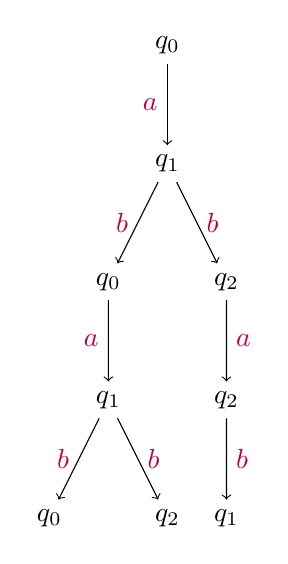
\begin{tikzpicture}
			\node {$q_0$}
			child { node {$q_1$} 
						child {node {$q_0$}
							child {node {$q_1$}
								child {node {$q_0$}
									edge from parent [->] node [left, purple] {$b$}
								}
								child {node {$q_2$}
									edge from parent [->] node [right, purple] {$b$}
								}
								edge from parent [->] node [left, purple] {$a$}
							}
							edge from parent [->] node [left, purple] {$b$}
						}
						child {node {$q_2$}
							child {node {$q_2$}
								child {node {$q_1$}
									edge from parent [->] node [right, purple] {$b$}
								}
								edge from parent [->] node [right, purple] {$a$}
							}
							edge from parent [->] node [right, purple] {$b$}
						}
						edge from parent [->] node [left, purple] {$a$}
			}
			;
		\end{tikzpicture}
		\caption{Árvore de computação da palavra ``$abab$'' no AFN da Figura \ref{fig:AFN1}.}
		\label{fig:ArvoreComputacaoAFN}
	\end{figure}
\end{exemplo}

Outra forma de visualizar a evolução de um AFN (ou AFD) durante o processamento de uma palavra $w \in \Sigma^*$ é usando a ideia de descrição instantânea (ou descrição de momento).

%\begin{definicao}
%	Uma descrição instantâne (DI) de um AFN (ou AFD) $A = \langle Q, \Sigma, \delta_N, q_0, F\rangle$, é uma palavra $uqv \in (Q \cup \Sigma)^*$, descreve como o autômato está em algum momento do processamento de uma palavra $w \in \Sigma^*$, onde $w = uv$, e o primento símbolo em $v$ corresponde ao símbolo que está sendo lido pela cabeçote na memória do autômato.
%\end{definicao}

%\begin{exemplo}
%	Considere AFN ilustrado na Figura \ref{fig:AFN1} antes de iniciar o processamento da palavra $bab$ o AFN está na DI $q_0bab$, após processar o primeiro $b$, o autômato se encontra na DI $bq_1ab$.
%\end{exemplo}

Pode-se agora apresentar a noção de aceitação (reconhecimento ou computação) de palavras nos AFD.

\begin{definicao}[Reconhecimento de palavras em AFN]\label{defi:PalavraAceitaPorAFN}
	Sejam $A = \langle Q, \Sigma, \delta_N, q_0, F\rangle$ um AFN e seja $w \in \Sigma^*$. A palavra $w$ é dita aceita (reconhece ou computada) por $A$ sempre que $\widehat{\delta}(q_0, w) \cap F \neq \emptyset$ e é rejeitada por $A$ em qualquer outro caso.
\end{definicao}

Note que a Definição \ref{defi:PalavraAceitaPorAFN} pode ser informalmente interpretada da seguinte forma, uma palavra é aceita por um AFN $A$ se existe pelo menos um caminho de computação para $w$ que termine em um estado final, isto é, pelo menos uma das folhas na árvore de computação deve ser um estado $q \in F$, neste caso $w$ é aceita por $A$.

\begin{exemplo}\label{exe:AceitacaoEmAFN}
	Considerando o AFN representado pela Figura \ref{fig:AFN2} a seguir e as palavras ``$aabbbba$'' e ``$aabb$'' tem-se que: 
	$$\widehat{\delta_N}(q_0, aabbbba) = \{q_1, q_3\}$$ 
	e  
	$$\widehat{\delta_N}(q_0, aabb) = \{q_2, q_3\}$$ 
	logo a palavra ``$aabbbba$'' é aceita por tal AFN. Por outro lado, a palavra ``$aabb$'' não é aceita pelo AFN.
	
	\begin{figure}[H]
		\centering
		\begin{tikzpicture}[>=stealth, shorten >=1pt, node distance=3.0cm, on grid, auto, state/.append style={minimum size=3em}, thick ]
			\node[state, initial]				(A)               	{$q_0$};
			\node[state, accepting]				(B) [right of=A] 	{$q_1$};
			\node[state]				        (C) [right of=B] 	{$q_2$};
			\node[state]				        (D) [right of=C] 	{$q_3$};
			\path[->] (A) +(-1,0) edge (A)
			
			%Transições:
			%(Partida) edge [tipo da seta] node {simbolo lido} (Destino)
			(A) edge 			 				node [below] {$a$}		 (B)
			(A) edge [loop above]  				node 		 {$a$}		 ( )
			(B) edge 			  				node [above] {$b$}		 (C)
			(C) edge [loop above]  				node 		 {$b$}		 ( )
			(C) edge 			  				node [above] {$b$}		 (D)
			(D) edge [loop above]  				node 		 {$a$}		 ( )
			(D) edge [bend left]  				node [below] {$a$}		 (B);
		\end{tikzpicture}
		\caption{Grafo de transição de um AFN.}
		\label{fig:AFN2}
	\end{figure}
\end{exemplo}

Usando a definição apresentada anteriormente de palavra aceita pode-se finalmente introduzir formalmente a noção de linguagem aceita (computada ou reconhecida) pelos AFN.

\begin{definicao}[Linguagem de um AFN]\label{def:LinguagemAFN}
	Seja $A = \langle Q, \Sigma, \delta_N, q_0, F\rangle$ um AFN a linguagem reconhecida (ou computada) por $A$, denotada por $\mathcal{L}(A)$, corresponde ao conjunto de todas as palavras aceitas por $A$, formalmente tem-se que:
	\begin{eqnarray}
		\mathcal{L}(A) = \{w \in \Sigma^* \mid \widehat{\delta_N}(q_0, w) \cap F \neq \emptyset\}
	\end{eqnarray}
\end{definicao}

De forma similar ao que ocorre com os AFD, para mostrar que uma linguagem $L$ é aceita por algum AFN $A$ deve-se provar a igualdade $L = \mathcal{L}(A)$, ou seja, deve-se provar que $w \in L \Longleftrightarrow w \in \mathcal{L}(A)$.

\begin{exemplo}\label{exe:LinguagemAFN1}
	A linguagem $L = \{a^i(ba)^j \mid i \geq 1,j \geq 0\}$ é aceita pelo AFN $A$ representado pelo grafo de transição da Figura \ref{fig:AFN3} a seguir.

  \begin{figure}[H]
		\centering
		\begin{tikzpicture}[>=stealth, shorten >=1pt, node distance=3.0cm, on grid, auto, state/.append style={minimum size=3em}, thick ]
			\node[state, initial]				(A)               	{$s_0$};
			\node[state, accepting]				(B) [right of=A] 	{$s_1$};
			\node[state]				        (C) [right of=B] 	{$s_2$};
			\path[->] (A) +(-1,0) edge (A)
			
			%Transições:
			%(Partida) edge [tipo da seta] node {simbolo lido} (Destino)
			(A) edge [loop above]  				node 		 {$a$}		 ( )
			(A) edge 			  				node 		 {$a$}		 (B)
			(B) edge [bend left]  				node 		 {$b$}		 (C)
			(C) edge [bend left]  				node 		 {$a$}		 (B);
		\end{tikzpicture}
		\caption{Grafo de transição de um AFN.}
		\label{fig:AFN3}
	\end{figure}
\end{exemplo}

\begin{prova}
	$(\Rightarrow)$ Suponha que $w \in L$, portanto, $w = a^m(ba)^n$,  e agora por indução dupla sobre o par $(m,n)$ tem-se que:
	\begin{itemize}
		\item[ ] \textbf{(B)}ase: Quando com $m = 1$ e $n = 0$ vale a igualdade $w = a^1(ba)^0 = a$, agora usando a definição de $\delta_N$ do AFN $A$ como representado na Figura \ref{fig:AFN3} tem-se que, 
		\begin{eqnarray*}
			\widehat{\delta_N}(s_0, a) = \bigcup_{s' \in \widehat{\delta}(s_0, \lambda)} \delta_N(s', a) = \delta_N(s_0, a) = \{s_0, s_1\}
		\end{eqnarray*}
		uma vez que, $s_1 \in F$ tem-se que $\widehat{\delta_N}(s_0, a) \cap F \neq \emptyset$, e portanto, $w \in \mathcal{L}(A)$. Agora suponha que para $w = a^1(ba)^n$ com $n \geq 0$ tem-se que $\widehat{\delta_N}(s_0, a^1(ba)^n) \cap F \neq \emptyset$. Assim dado $a^1(ba)^{n+1}$ por definição tem-se que:
		\begin{eqnarray}\label{eq:ProvaAFNLinguagem1}
			\widehat{\delta_N}(s_0, a^1(ba)^{n+1}) & = & \widehat{\delta_N}(s_0, a^1(ba)^{n}ba)\nonumber\\
			& = & \bigcup_{s' \in \widehat{\delta_N}(s_0, a^1(ba)^{n}b)} \delta_N(s', a)
		\end{eqnarray}
		agora fazendo,
		\begin{eqnarray}\label{eq:ProvaAFNLinguagem2}
			K = \bigcup_{s'' \in \widehat{\delta_N}(s_0, a^1(ba)^{n})} \delta_N(s'', b)
		\end{eqnarray}
		e reescrevendo a Equação (\ref{eq:ProvaAFNLinguagem1}) usando a Equação (\ref{eq:ProvaAFNLinguagem2}) tem-se que,
		\begin{eqnarray}\label{eq:ProvaAFNLinguagem3}
			\widehat{\delta_N}(s_0, a^1(ba)^{n+1}) & = & \bigcup_{s' \in K} \delta_N(s', a)
		\end{eqnarray}
		entretanto, por hipótese tem-se que $\widehat{\delta_N}(s_0, a^1(ba)^n) \cap F \neq \emptyset$, consequentemente, tem-se que $s_1 \in \widehat{\delta_N}(s_0, a^1(ba)^n)$ dessa forma pela Equação (\ref{eq:ProvaAFNLinguagem2}) é claro que $\delta_N(s_1, b) \subseteq K$. Mas $\delta_N(s_1, b) = \{s_2\}$ logo pela Equação (\ref{eq:ProvaAFNLinguagem3}) tem-se que $\delta_N(s_2, a) \subseteq \widehat{\delta_N}(s_0, a^1(ba)^{n+1})$, desde que $\delta_N(s_2, a) = \{s_1\}$, tem-se $s_1 \in \widehat{\delta_N}(s_0, a^1(ba)^{n+1})$, portanto, $\widehat{\delta_N}(s_0, a^1(ba)^{n+1}) \cap F \neq \emptyset$, consequentemente $a^1(ba)^{n+1} \in \mathcal{L}(A)$.

		\item[ ] \textbf{(H)}ipótese indutiva: Assuma que $\widehat{\delta_N}(s_0, a^m(ba)^n)  \cap F \neq \emptyset$ com $n \geq 0$.
		\item[ ] \textbf{(P)}asso indutivo: Primeiro seja $w \in L$ de forma que $w = a^{m+1}(ba)^0$ logo pela hipótese indutiva segue que,
		\begin{eqnarray*}
			\widehat{\delta_N}(s_0, a^{m+1}(ba)^0) \cap F \neq \emptyset
		\end{eqnarray*}
		consequentemente, $a^{m+1}(ba)^0 \in \mathcal{L}(A)$. Além disso, sendo $w \in L$ tal que $w = a^{m+1}(ba)^n$, usando a  definição de $\widehat{\delta_N}$ tem-se para $a^{m+1}(ba)^{n+1}$ que, 
		\begin{eqnarray}\label{eq:ProvaAFNLinguagem4}
			\widehat{\delta_N}(s_0, a^{m+1}(ba)^{n+1}) & = & \widehat{\delta_N}(s_0, a^{m+1}(ba)^{n}ba)\nonumber\\
			& = & \bigcup_{s' \in \widehat{\delta_N}(s_0, a^{m+1}(ba)^{n}b)} \delta_N(s', a)
		\end{eqnarray}
		agora desenvolvendo o termo $\widehat{\delta_N}(s_0, a^{m+1}(ba)^{n}b)$ tem-se
		\begin{eqnarray*}
			\widehat{\delta_N}(s_0, a^{m+1}(ba)^{n}b) & = & \bigcup_{s'' \in \widehat{\delta_N}(s_0, a^{m+1}(ba)^{n})} \delta_N(s'', b)
		\end{eqnarray*}
		por \textbf{(H)} tem-se que $\widehat{\delta_N}(s_0, a^{m+1}(ba)^{n}) \cap F = \emptyset$, consequentemente, tem-se $s_1 \in \widehat{\delta_N}(s_0, a^{m+1}(ba)^{n})$, e dessa forma é claro que a relação de inclusão, $\delta_N(s_1, b) \subseteq \widehat{\delta_N}(s_0, a^{m+1}(ba)^{n})$ acontece. Agora, uma vez que, $\delta_N(s_1, b) = \{s_2\}$, tem-se que $\{s_2\} \subseteq \widehat{\delta_N}(s_0, a^{m+1}(ba)^{n})$, assim pela Equação (\ref{eq:ProvaAFNLinguagem4}) segue que $\delta_N(s_2, a) \subseteq \widehat{\delta_N}(s_0, a^{m+1}(ba)^{n+1})$, mas por definição $\delta_N(s_2, a) = \{s_1\}$, portanto, tem-se que $\{s_1\} \subseteq \widehat{\delta_N}(s_0, a^{m+1}(ba)^{n+1})$, logo $\widehat{\delta_N}(s_0, a^{m+1}(ba)^{n+1}) \cap F \neq \emptyset$ e assim $a^{m+1}(ba)^{n+1} \in \mathcal{L}(A)$.
	\end{itemize}
	Consequentemente por \textbf{(B), (H)} e \textbf{(P)} segue que $\widehat{\delta_N}(s_0, a^{m}(ba)^{n}) \cap F \neq \emptyset$ para todo $m \geq 1$ e $n \in \mathbb{N}$.

	$(\Leftarrow)$ Suponha que $w \in \mathcal{L}(A)$ assim $s_1 \in \widehat{\delta_N}(s_0, w)$, note porém que $s_1$ só é acessível a partir de duas transições: 
	\begin{itemize}
		\item[(1)] $\delta_N(s_0, a)$ e
		\item[(2)] $\delta_N(s_2, a)$. 
	\end{itemize}
	Note que devido ao \textit{loop} fornecido pelo fato de que $s_0 \in \delta_N(s_0, a)$ a transição (1) pode ser executada $m$ vezes com $m \geq 1$, em que para cada execução um novo ramo com o estado $s_1$ é gerado na árvore de computação de $A$, entretanto, executar $m$ vezes a transição $\delta_N(s_0, a)$ implica em executar a computação $\widehat{\delta_N}(s_0, a^m)$, pelo fato\footnote{Fica para o leitor a tarefa de provar que para todo $m \geq 1$ tem-se que $s_1 \in \widehat{\delta_N}(s_0, a^m)$.} de que $s_1 \in \widehat{\delta_N}(s_0, a^m)$ tem-se que $a^m \in \mathcal{L}(A)$, e uma vez que $a^m = a^m(ba)^0$ tem-se que a primeira forma de $\widehat{\delta_N}(s_0, w) \cap F \neq \emptyset$ é que $w = a^m(ba)^0$ e assim $w \in L$. Por outro lado, para acessar $s_1$ via a transição (2) é necessário antes chegar a um ramo de computação em que o estado $s_2$ seja uma folha, mas pela definição de $A$ isso só é possível se a transição $\delta_N(s_1, b)$ for usada, note entretanto, que as transições $\delta_N(s_1, b) = \{s_2\}$ e $\widehat{\delta_N}(s_2, a) = \{s_1\}$ também geram um \textit{loop} que pode ser executado $n$ vezes com $n \geq 0$, mas executar esse \textit{loop} $n$ vezes corresponde a executar $\widehat{\delta_N}(s_1, (ba)^n)$, e como dito anteriormente, $s_1$ só é acessível pela definição de $A$ usando a computação $\widehat{\delta_N}(s_0, a^m)$, portanto, para que $s_1 \in \widehat{\delta_N}(s_0, w) \cap F$, obrigatoriamente, $w = a^m(ba)^n$ com $m \geq 1, n \geq 0$, e portanto, $w \in L$.
\end{prova}

\begin{figure}[H]
  \centering
  \begin{tikzpicture}[>=stealth, shorten >=1pt, node distance=3.0cm, on grid, auto, state/.append style={minimum size=3em}, thick ]
    \node[state, initial]						(A)               	{$s_0$};
    \node										(B) [right of=A] 	{ };
    \node[state, accepting]				        (C) [above of=B] 	{$s_1$};
    \node[state, accepting]				        (D) [below of=B] 	{$s_2$};
    \path[->] (A) +(-1,0) edge (A)
    
    %Transições:
    %(Partida) edge [tipo da seta] node {simbolo lido} (Destino)
    (A) edge [loop above]  				node 		 {$0, 1$}		 ( )
    (A) edge							node 		 {$0$}			 (C)
    (A) edge							node 		 {$1$}			 (D);
  \end{tikzpicture}
  \caption{Grafo de transição de um AFN $S$.}
  \label{fig:AFN4}
\end{figure}

\begin{exemplo}\label{exe:LinguagemAFN2}
	O AFN $S$ representado no grafo de transição exposto na Figura \ref{fig:AFN4} a seguir reconhece a linguagem $L = \{uv \mid u \in \{0,1\}^*,  v \in \{0,1\}\}$.
\end{exemplo}

\begin{prova}
	$(\Rightarrow)$ A ida fica a cargo do leitor. $(\Leftarrow)$ Suponha que $w \in \mathcal{L}(A)$ assim por definição $\widehat{\delta_N}(s_0, w) \cap \{s_1, s_2\} \neq \emptyset$, agora pela definição de $\delta_N$ é claro que toda árvore de computação de $A$ apresenta a propriedade de sempre conter um dos estados $s_1$ ou $s_2$, mas nunca os dois simultaneamente\sidefootnote{A prova desta propriedade fica como exercício ao leitor.}. Além disso, o fato de
	$$s_0 \in \widehat{\delta_N}(s_0, a)$$
	para todo $a \in \{0,1\}$, garante que qualquer palavra não a vazia $u$ sobre o alfabeto $\{0,1\}$ pode ser gerada, por fim, no último passo de computação é claro que $s_1$ ou $s_2$ será uma folha da árvore, entretanto, $s_1$ só será tal folha no caso da palavra terminar em $0$ caso contrário a folha será $s_2$, e portanto, todo $w \in \mathcal{L}(A)$ tem a foma $uv$ com $u \in \{0, 1\}^*$ e $v \in \{0,1\}$, consequentemente $w \in L$.
\end{prova}

De forma ingênua o leitor pode vim a imaginar que a possibilidade da unidade de controle de um AFN poder assumir mais de um estado interno simultaneamente, faz com que os AFN sejam mais poderosos que os AFD, entretanto, como será exibido pelos resultados a seguir, isso não ocorre, de fato, como dito \cite{benjaLivro2010, linz2006} apesar de tornar mais fácil a tarefa de construir um autômato quem reconheça uma linguagem $L$, o não-determinismo não aumenta nem nada o poder de computação dos autômatos finitos.

\begin{teorema}[Transformação AFD - AFN]\label{teo:AFD-Para-AFN}
	Se $L = \mathcal{L}(A)$ para algum AFD $A$, então existe um AFN $A'$ tal que $L = \mathcal{L}(A')$.
\end{teorema}

\begin{prova}
	A prova é trivial, uma vez que, todo AFD $A = \langle Q, \Sigma, \delta, q_0, F\rangle$ pode ser convertido em um AFN $A' = \langle Q, \Sigma, \delta_N, q_0, F\rangle$ apenas realizando as transformações das transições $\delta(q_i, a) = q_j$ nas transições não-determinísticas $\delta_N(q_i, a) = \{q_j\}$ e mantendo todo o resto da estrutura igual.
\end{prova}

O próximo resultado estabelece a contraparte do Teorema \ref{teo:AFD-Para-AFN}, isto é, tal resultado mostrará que sempre é possível obter um AFD que pode ``simular''. O termo simular aqui, diz respeito a ideia de que cada aplicação de uma função de transição não-determinística pode ser representada de forma precisa por uma aplicação de uma função de transição determinística, para detalhes consulte \cite{hopcroft2008, menezes1998LFA}.

\begin{teorema}[Transformação AFN - AFD]\label{teo:AFN-Para-AFD}
	Se $L = \mathcal{L}(A)$ para algum AFN $A$, então existe um AFD $A'$ tal que $L = \mathcal{L}(A')$.
\end{teorema}

\begin{prova}
	Suponha que $L = \mathcal{L}(A)$ para algum AFN $A = \langle Q, \Sigma, \delta_N, q_0, F\rangle$, agora é construído um  autômato $A' = \langle \wp(Q), \Sigma, \delta, \{q_0\}, F' \rangle$ onde para todo $X \in \wp(Q)$ e $a \in \Sigma$ tem-se
	\begin{eqnarray}\label{eq:TranformacaoDelta-DeltaN}
		\delta(X, a) = \bigcup_{q \in X} \delta_N(q, a)
	\end{eqnarray}
	claramente este autômato é realmente determinístico, e para todo $X \in \wp(Q)$  tem-se que $X \in F'$ se, e somente se, $X \cap F \neq \emptyset$. Agora será mostrado por indução sobre o tamanho de $w \in \Sigma^*$ que:
	$$\widehat{\delta}(\{q_0\}, w) = \widehat{\delta_N}(q_0, w)$$
	\begin{itemize}
		\item[ ] \textbf{(B)}ase: Quando $|w| = 0$ isto é $w = \lambda$ tem-se trivialmente pela definição das funções de transição estendidas que $\widehat{\delta}(\{q_0\}, \lambda) = \widehat{\delta_N}(q_0, \lambda)$.
		
		\item[ ] \textbf{(H)}ipótese indutiva: Suponha que para todo $w \in \Sigma^*$ com $|w| \geq 0$ tem-se que $\widehat{\delta}(\{q_0\}, w) = \widehat{\delta_N}(q_0, w)$.
		\item[ ] \textbf{(P)}asso indutivo: Dado $w = ua$ com $u \in \Sigma^*$, $|u| \geq 0$ e $a \in \Sigma$ tem-se que, 
		\begin{eqnarray*}
			\widehat{\delta}(\{q_0\}, w) & = & \widehat{\delta}(\{q_0\}, ua)\\
			& = & \delta(\widehat{\delta}(\{q_0\}, u), a)\\
			& \stackrel{\textbf{(HI)}}{=} & \delta(\widehat{\delta_N}(q_0, u), a)\\
			& \stackrel{Eq. (\ref{eq:TranformacaoDelta-DeltaN})}{=} & \bigcup_{q \in \widehat{\delta_N}(q_0, u)} \delta_N(q, a)\\
			& = & \widehat{\delta_N}(q_0, ua)\\
			& = & \widehat{\delta_N}(q_0, w)
		\end{eqnarray*}
	\end{itemize}
	Portanto, pode-se concluir por \textbf{(B)}, \textbf{(H)} e \textbf{(P)} que $w \in \mathcal{L}(A)$ se, e somente se, $w \in \mathcal{L}(A')$, ou seja, $L = \mathcal{L}(A')$ o que completa a prova.
\end{prova}

Observe que o método de construção usado na prova do Teorema \ref{teo:AFN-Para-AFD} cria um AFD cujo número de estado cresce em razão de uma potência de 2 quando comparado com o quantitativo de estados do AFN original. Como consequência deste resultado segue o seguinte corolário.

\begin{corolario}
  Uma linguagem $L$ é regular se, e somente se, existe um AFN $A$ tal que $L = \mathcal{L}(A)$.
\end{corolario}

\begin{prova}
	$(\Rightarrow)$ Assuma que $L$ é regular, assim por definição existe um AFD $A'$ tal que $L = \mathcal{L}(A')$, entretanto, pelo Teorema \ref{teo:AFD-Para-AFN} existe um AFN $A$ tal que $L = \mathcal{L}(A)$. $(\Leftarrow)$ Suponha que $L = \mathcal{L}(A)$ para algum AFN $A$, agora pelo Teorema \ref{teo:AFN-Para-AFD} existe um AFD $A'$ tal que $L = \mathcal{L}(A')$, e portanto, por definição $L$ é regular.
\end{prova}

É importante destacar que o método de construção do AFD usado na prova do Teorema \ref{teo:AFN-Para-AFD}, conhecido como método de construção das partes introduzido por Rabin e Scott em \cite{rabin1959}, tem a característica de poder vim a produzir durante sua execução alguns estados inacessíveis\sidefootnote{Um estado $q$ em um AFD é dito inacessível se não existe um $w \in \Sigma^*$ tal que $\widehat{\delta}(q_0, w) = q$. Vale também ressaltar como destaco em \cite{benjaLivro2010, hopcroft2008} que estados inacessíveis não aumentam o poder de computação nos AFD.} no AFD resultante.

Outro ponto sobre o método de construção das partes é que em alguns cenários pode ser tornar impraticável, pois se o AFN de entrada possuir $n$ estados, o AFD resultante do método terá $2^n$ estados, ou seja, o crescimento no número de estados do AFD resultante do método cresce proposicional a uma potência de 2, o que rapidamente gera um número exponencialmente grande de estados. 

%A seguir o leitor será apresentado a uma melhoria no algoritmo de construção das partes, no sentido de que, a execução de tal algoritmo não produz estados inacessíveis no AFD de saída, o algoritmo a seguir é um pseudo-código baseado na versão textual apresentada no livro de Bedregal \textit{et al.} \cite{benjaLivro2010}. A melhoria no Algoritmo \ref{alg:AFN-AFD} consiste do fato dele não considerar simplesmente o conjunto $\wp(Q)$ no AFD de saída, em vez disso, ele constrói interativamente um conjunto de estados $Q' \subseteq \wp(Q)$, que no pior caso\sidefootnote{A expressão ``no pior caso'' é típica da análise de algoritmos, em momentos futuros essa ideia de pior caso será melhor desenvolvida neste manuscrito.} tem-se que $Q' = \wp(Q)$.

A seguir o leitor será apresentado a uma melhoria no algoritmo de construção das partes, no sentido de que, a execução de tal algoritmo não produz estados inacessíveis no AFD de saída, o algoritmo a seguir é um pseudo-código baseado na versão textual apresentada no livro de Bedregal \textit{et al.} \cite{benjaLivro2010}. A melhoria no Algoritmo \ref{alg:AFN-AFD} consiste do fato dele não considerar simplesmente o conjunto $\wp(Q)$ no AFD de saída, em vez disso, ele constrói interativamente um conjunto de estados $Q' \subseteq \wp(Q)$, que no pior caso tem-se que $Q' = \wp(Q)$.

\begin{algorithm}[H]
	\Entrada{Um AFN $A = \langle Q, \Sigma, \delta_N, q_0, F\rangle$}
	\Saida{Um AFD $A' = \langle Q', \Sigma, \delta, \{q_0\}, F' \rangle$}
	\Inicio{
		Inicialize os conjuntos $Q_u$ e $Q'$ com um  estado rotulado por $\{q_0\}$\\
		Inicialize o conjunto $F'$ como sendo vazio\\
		\Repita{$Q_u = \emptyset$}{
			Selecione um estado $X \in Q_u$\\
			\ParaCada{$a \in \Sigma$}{
				Determine o conjunto $\displaystyle Y = \bigcup_{q \in X}\delta_N(q, a)$\\
				\Se{$Y \notin Q'$}{
					Adicione o estado rotulado por $Y$ em $Q'$ e em $Q_u$\\
				}
        Defina a transição $\delta(X, a) = Y$\\
			}
			Remova $X$ de $Q_u$
		}
		\ParaCada{$X \in Q'$}{
			\Se{$X \cap F \neq \emptyset$}{
				Adicione $X$ ao conjunto $F'$
			}
		}
		\Retorna{$A' = \langle Q', \Sigma, \delta, \{q_0\}, F' \rangle$}
	}
	\caption{Algoritmo para converter AFN em AFD sem estados inacessíveis.}
	\label{alg:AFN-AFD}
\end{algorithm}

\begin{exemplo}\label{exe:ConvertendoAFN-AFD}
	Usando o Algoritmo \ref{alg:AFN-AFD}  tendo o AFN representado pelo grafo de transição da Figura \ref{fig:AFN2} como entrada será obtido o AFD $M = \langle \{s_0, s_1, s_2, s_3, $ $s_4, \emptyset\}, \{a,b\}, \delta, s_0, F'\rangle$, onde tem-se os estados equivalem aos seguintes conjuntos,
	\begin{eqnarray*}
		s_0 & = & \{q_0\}\\
		s_1 & = & \{q_0, q_1\}\\
		s_2 & = & \{q_2\}\\
		s_3 & = & \{q_2, q_3\}\\
		s_4 & = & \{q_1, q_3\}
	\end{eqnarray*} 
	tem-se que $F' = \{s_1, s_4\}$ e a função de transição $\delta$ é como se segue.

  \begin{table}[H]
    \centering
    \begin{tabular}{c|cc}
      \diagbox{$Q$}{$\Sigma$}	& $a$ & $b$\\ \hline
      $s_0$ & $s_1$ & $\emptyset$\\
      $s_1$ & $s_1$ & $s_2$\\
      $s_2$ & $\emptyset$ & $s_3$\\
      $s_3$ & $s_4$ & $s_3$\\
      $s_4$ & $s_4$ & $s_2$\\
      $\emptyset$ & $\emptyset$ & $\emptyset$\\ \hline
    \end{tabular}
    \caption{Tabela da função de transição do AFD $M$ obtido a partir do uso do Algoritmo \ref{alg:AFN-AFD} no AFN da Figura \ref{fig:AFN2}.}
  \end{table}
\end{exemplo}

\section{$\lambda$-Autômatos Finitos Não-determinísticos}\label{subsec:LAFN}

Os $\lambda$-Autômatos Finitos Não-determinísticos, ou simplesmente, $\lambda$-AFN são como dito em \cite{menezes1998LFA}, uma generalização do modelo de AFN que foi introduzido na seção anterior e que são permitidas transições entre estados diferentes usando (ou consumindo) a palavra vazia, tais transições recebem o nome de $\lambda$-transições, a seguir tais autômatos serão apresentados formalmente.

\begin{definicao}[$\lambda$-Autômatos Finitos Não-determinísticos]\label{def:LAFN}
	Um $\lambda$-AFN é uma estrutura $A = \langle Q, \Sigma, \underline{\delta_N}, q_0, F\rangle$ onde: $Q, \Sigma, q_0$ e $F$ são da mesma forma que na Definição \ref{def:AFD}, já $\underline{\delta_N} : Q \times (\Sigma \cup \{\lambda\}) \rightarrow \wp(Q)$ é uma função total (chamada $\lambda$-função de transição não determinística).
\end{definicao}

A representação usando grafos de transição dos $\lambda$-AFN e similar a representação dos AFN da seção anterior, a única diferença é que podem haver transições rotuladas pelo símbolo $\lambda$, isto é, podem existir no grafo arestas entre vértices que são rotuladas por $\lambda$, e o mesmo vale para a representação das árvores de computação.

\begin{exemplo}\label{exe:LAFN1}
	A estrutura $A = \langle \{q_0, q_1, q_2\}, \{0,1\}, \underline{\delta_N}, q_0, \{q_0\}\rangle$ com $\underline{\delta_N}$ sendo especificada pela Tabela \ref{tab:DeltaLAFN1} a seguir é um $\lambda$-AFN.
	
	\begin{table}[H]
		\centering
		\begin{tabular}{c|ccc}
			\backslashbox{$Q$}{$\Sigma \cup \{\lambda\}$}	& $0$ & $1$ & $\lambda$\\ \hline
			$q_0$  & $\emptyset$ & $\emptyset$ & $\{q_1\}$\\
			$q_1$  & $\{q_1\}$ & $\{q_2\}$ & $\{q_2\}$\\
			$q_2$  & $\{q_2\}$ & $\{q_2\}$ & $\{q_0, q_2\}$ \\ \hline
		\end{tabular}
		\caption{Tabela de transição para a função $\underline{\delta_N}$ do AFN no Exemplo \ref{exe:LAFN1}.}
		\label{tab:DeltaLAFN1}
	\end{table}
\end{exemplo} 


\begin{exemplo}\label{exe:LAFN-linguagem}
	O $\lambda$-AFN $A = \langle \{q_0, q_1, q_2\}, \{0, 1\}, \underline{\delta_N}, q_0, \{q_2\} \rangle$ com $\underline{\delta_N}$ sendo especificada pela Tabela \ref{tab:DeltaLAFN-linguagem1} a seguir é um $\lambda$-AFN.
	
	\begin{table}[H]
		\centering
		\begin{tabular}{c|ccc}
			\backslashbox{$Q$}{$\Sigma \cup \{\lambda\}$}	& $0$ & $1$ & $\lambda$\\ \hline
			$q_0$  & $\emptyset$ & $\emptyset$ & $\{q_1\}$\\
			$q_1$  & $\{q_1\}$ & $\emptyset$ & $\{q_2\}$\\
			$q_2$  & $\emptyset$ & $\{q_2\}$ & $\emptyset$ \\ \hline
		\end{tabular}
		\caption{Tabela de transição para a função $\underline{\delta_N}$ do AFN no Exemplo \ref{exe:LAFN-linguagem}.}
		\label{tab:DeltaLAFN-linguagem1}
	\end{table}

	e representado pela figura \ref{fig:LAFN-linguagem} a seguir. 


	\begin{figure}[H]
		\centering
		\begin{tikzpicture}[>=stealth, shorten >=1pt, node distance=2.5cm, on grid, auto, state/.append style={minimum size=3em}, thick ]
			\node[state, initial]									(A)               	{$q_0$};
			\node[state]													(B) [right of=A] 	{$q_1$};
			\node[state, accepting]				        (C) [right of=B] 	{$q_2$};
			\path[->] (A) +(-1,0) edge (A)
			
			%Transições:
			%(Partida) edge [tipo da seta] node {simbolo lido} (Destino)
			(A) edge											node 		 {$\lambda$} (B)
			(B) edge [loop above]  				node 		 {$0$} 		 ( )
			(C) edge [loop above]  				node 		 {$1$} 		 ( )
			(B) edge											node 		 {$\lambda$} (C);
		\end{tikzpicture}
		\caption{Grafo de transição do $\lambda$-AFN do Exemplo \ref{exe:LAFN-linguagem}.}
		\label{fig:LAFN-linguagem}
	\end{figure}
\end{exemplo}

\begin{exemplo}
	O grafo de transição representado na Figura \ref{fig:LAFN1} a seguir é uma representação para o $\lambda$-AFN do Exemplo \ref{exe:LAFN1}.
	
	\begin{figure}[H]
		\centering
		\begin{tikzpicture}[>=stealth, shorten >=1pt, node distance=2.5cm, on grid, auto, state/.append style={minimum size=3em}, thick ]
			\node[state, initial, accepting]	(A)               	{$q_0$};
			\node[state, accepting]				(B) [right of=A] 	{$q_1$};
			\node[state]				        (C) [right of=B] 	{$q_2$};
			\path[->] (A) +(-1,0) edge (A)
			
			%Transições:
			%(Partida) edge [tipo da seta] node {simbolo lido} (Destino)
			(A) edge							node 		 {$\lambda$} (B)
			(B) edge							node [above] {$1, \lambda$} (C)
			(B) edge [loop above]  				node 		 {$0$} 		 ( )
			(C) edge [loop above]  				node 		 {$1, 0, \lambda$} ( )
			(C) edge [bend left]  				node [below] {$\lambda$} (A);
		\end{tikzpicture}
		\caption{Grafo de transição do $\lambda$-AFN do Exemplo \ref{exe:LAFN1}.}
		\label{fig:LAFN1}
	\end{figure}
\end{exemplo}

Uma interpretação para as transições da forma $\underline{\delta_N}(q, \lambda) = X$ é que a unidade de controle do autômato consegue mudar seu estado interno $q$ para um subconjunto de estados $X$ sem precisar acessar a memória.

Note porém que a definição da função de transição $\underline{\delta_N}$ garante que as transições em um $\lambda$-AFN acontecem apenas em duas situações, a primeira em relação símbolos individuais do alfabeto $\Sigma$ e a segunda com relação a palavra vazia, assim não existe uma forma de computar uma palavra $w$ de forma que $|w| > 1$. A saída para contorna esse fato é estender a função de transição do autômato, similarmente ao que é feito para os AFD e AFN, para isso entretanto, é necessária algumas definições adicionais.

\begin{definicao}[Função $\delta_\lambda$]\label{def:L-fecho}
	Seja $A = \langle Q, \Sigma, \underline{\delta_N}, q_0, F\rangle$ um $\lambda$-AFN, então a função $\delta_\lambda: Q \rightarrow \wp(Q)$ é definida como,
	\begin{equation}
		\delta_\lambda(q) = \bigcup_{i = 0}^n\lambda\text{-fecho}^i(q)
	\end{equation}
	onde $n = \# Q - 1$ e
	\begin{eqnarray}
		\lambda\text{-fecho}^0(q) & = & \{q\}\\
		\lambda\text{-fecho}^{i+1}(q) & = & \bigcup_{q' \in \lambda\text{-fecho}^{i}(q)} \underline{\delta_N}(q', \lambda)
	\end{eqnarray}
\end{definicao}

\begin{exemplo}
	Considere o $\lambda$-AFN da Figura \ref{fig:LAFN-linguagem} tem-se para o estado $q_1$ que,
	\begin{eqnarray}\label{eq:LAFNeq1}
		\delta_\lambda(q_1) & = & \bigcup_{i = 0}^{2}\lambda\text{-fecho}^i(q_1) \nonumber\\
		& = & \lambda\text{-fecho}^2(q_1) \cup \lambda\text{-fecho}^1(q_1) \cup \lambda\text{-fecho}^0(q_1)  
	\end{eqnarray}
	sabe-se que, 
	\begin{eqnarray*}
		\lambda\text{-fecho}^{0}(q_1) & = &  \{q_1\}
	\end{eqnarray*}
	e desenvolvendo $\lambda\text{-fecho}^{2}(q_1)$ tem-se que,
	\begin{eqnarray*}
		\lambda\text{-fecho}^{2}(q_1) & = &  \bigcup_{q' \in \lambda\text{-fecho}^{1}(q_1)} \underline{\delta_N}(q', \lambda)
	\end{eqnarray*}
	mas, 
	\begin{eqnarray*}
		\lambda\text{-fecho}^{1}(q_1) & = & \bigcup_{q' \in \lambda\text{-fecho}^{0}(q_1)} \underline{\delta_N}(q', \lambda)\\
		& = & \bigcup_{q' \in \{q_1\}} \underline{\delta_N}(q', \lambda)\\
		& = & \{q_2\}
	\end{eqnarray*}
	assim,
	\begin{eqnarray*}
		\lambda\text{-fecho}^{2}(q_1)  =   \bigcup_{q' \in \{q_2\}} \underline{\delta_N}(q', \lambda) = \underline{\delta_N}(q_2, \lambda) = \emptyset 
	\end{eqnarray*}
	substituindo tais resultados na Equação \ref{eq:LAFNeq1} tem-se que, 
	\begin{eqnarray*}\label{eq:LAFNeq2}
		\delta_\lambda(q_1) & = &  \emptyset \cup \{q_2\} \cup \{q_1\} = \{q_1, q_2\}
	\end{eqnarray*}
\end{exemplo}

Uma interpretação semântica para a função $\delta_\lambda$ é que ela representa a resposta ao questionamento: ``Estando no estado $q$ e executando $n$ $\lambda$-transições qual subconjunto de estados a unidade central do autômato irá assumir?''. 

\begin{definicao}[Função $\widehat{\delta_\lambda}$]\label{def:L-Fecho}
	Seja $A = \langle Q, \Sigma, \underline{\delta_N}, q_0, F\rangle$ um $\lambda$-AFN, então a função $\widehat{\delta_\lambda}: \wp(Q) \rightarrow \wp(Q)$ é definida como,
	\begin{equation}
		\widehat{\delta_\lambda}(X) = \bigcup_{q \in X} \delta_\lambda(q)
	\end{equation}
\end{definicao}

\begin{exemplo}
	Considere o $\lambda$-AFN da Figura \ref{fig:LAFN1} tem-se para o conjunto $\{q_1, q_2\}$ que,
	\begin{eqnarray*}
		\widehat{\delta_\lambda}(\{q_1, q_2\}) & = & \bigcup_{q \in \{q_1, q_2\}} \delta_\lambda(q)\\
		& = & \delta_\lambda(q_1) \cup \delta_\lambda(q_2)\\
		& = & \{q_0, q_1, q_2\} \cup \{q_0, q_2, q_1\}\\
		& = & \{q_0, q_2, q_1\}
	\end{eqnarray*}
\end{exemplo}

Agora usando as definições de $\delta_\lambda$ e $\widehat{\delta_\lambda}$ pode-se apresentar a extensão da função de transição dos $\lambda$-AFN.

\begin{definicao}[$\lambda$-Transição não-determinística estendida]\label{def:FuncaoLDeltaNDEstendida}
	Dado um $\lambda$-AFN  $A = \langle Q, \Sigma, \underline{\delta_N}, q_0, F\rangle$, a função $\underline{\delta_N}$ é estendido para a função $\widehat{\underline{\delta_N}}: Q \times \Sigma^* \rightarrow \wp(Q)$ definida pela seguinte recursão:
	\begin{eqnarray}\label{eq:FuncaoLDeltaNDEstendida}
		\widehat{\underline{\delta_N}}(q, \lambda)& = &  \delta_\lambda(q)\\
		\widehat{\underline{\delta_N}}(q, wa) & = & \bigcup_{q' \in \widehat{\underline{\delta_N}}(q, w)} \widehat{\delta_\lambda}(\underline{\delta_N}(q', a))
	\end{eqnarray}
\end{definicao}

\begin{exemplo}
	Considere o $\lambda$-AFN da Figura \ref{fig:LAFN1} tem-se a seguinte computação para a palavra ``$10$'':
	\begin{eqnarray}\label{eq:ExemLAFN1}
		\widehat{\underline{\delta_N}}(q_0, 10) & = & \bigcup_{q' \in \widehat{\underline{\delta_N}}(q_0, 1)} \widehat{\delta_\lambda}(\underline{\delta_N}(q', 0))\nonumber\\
		& = & \bigcup_{q' \in \widehat{\underline{\delta_N}}(q_0, 1)} \widehat{\delta_\lambda}(\underline{\delta_N}(q', 0))
	\end{eqnarray}
	mas,
	\begin{eqnarray}\label{eq:ExemLAFN2}
		\widehat{\underline{\delta_N}}(q_0, 1) & = & \bigcup_{q' \in \widehat{\underline{\delta_N}}(q_0, \lambda)} \widehat{\delta_\lambda}(\underline{\delta_N}(q', 1))\nonumber\\
		& = & \bigcup_{q' \in \delta_\lambda(q_0)} \widehat{\delta_\lambda}(\underline{\delta_N}(q', 1))\nonumber\\
		& = & \bigcup_{q' \in \{q_0, q_1, q_2\}} \widehat{\delta_\lambda}(\underline{\delta_N}(q', 1))\\
		& = & \widehat{\delta_\lambda}(\{q_1, q_2\})\nonumber\\
		& = & \{q_0, q_1, q_2\}\nonumber
	\end{eqnarray}
	substituindo o valor da Equação (\ref{eq:ExemLAFN2}) na Equação (\ref{eq:ExemLAFN1}) tem-se que, 
	\begin{eqnarray*}
		\widehat{\underline{\delta_N}}(q_0, 10) & = & \bigcup_{q' \in \{q_0, q_1, q_2\}} \widehat{\delta_\lambda}(\underline{\delta_N}(q', 0))\\
		& = & \{q_0, q_1, q_2\}
	\end{eqnarray*}
\end{exemplo}

Assim como para o caso dos AFN uma palavra qualquer $w \in \Sigma^*$ será dita aceita por um $\lambda$-AFN quando a computação da palavra $w$ para em pelo menos um estado final, ou seja, $w$ é reconhecida pelo $\lambda$-AFN sempre que $\widehat{\underline{\delta_N}}(q_0, w) \cap F \neq \emptyset$, e assim pode-se definir formalmente a noção de linguagem para os $\lambda$-AFN.

\begin{definicao}[Linguagem de um $\lambda$-AFN]\label{def:LinguagelLAFN}
	Seja $A = \langle Q, \Sigma, \underline{\delta_N}, q_0, F\rangle$ um $\lambda$-AFN a linguagem aceita por $A$, denotado por $\mathcal{L}(A)$, corresponde ao seguinte conjunto $\mathcal{L}(A) = \{w \in \Sigma^* \mid \widehat{\underline{\delta_N}}(q_0, w) \cap F \neq \emptyset\}$.
\end{definicao}

Os aspectos relacionados a mostrar que um $\lambda$-AFN reconhece uma linguagem $L$ são similares ao mesmo aspectos com respeito aos AFN.

\begin{exemplo}\label{exe:LinguagemLAFN1}
	O $\lambda$-AFN representado pelo grafo de transição da Figura \ref{fig:Linguagem-LAFN1} a seguir reconhece a linguagem $L = \{w \in \{1,2,3\}^* \mid w = 1^i2^j3^k \text{ com } i,j,k \in \mathbb{N}\}$.
	
	\begin{figure}[H]
		\centering
		\begin{tikzpicture}[>=stealth, shorten >=1pt, node distance=3.0cm, on grid, auto, state/.append style={minimum size=3em}, thick ]
			\node[state, initial]						(A)               	{$s_0$};
			\node[state]								(B) [right of=A] 	{$s_1$};
			\node[state, accepting]				        (C) [right of=B] 	{$s_2$};
			\path[->] (A) +(-1,0) edge (A)
			
			%Transições:
			%(Partida) edge [tipo da seta] node {simbolo lido} (Destino)
			(A) edge [loop above]  				node 		 {$1$} 		 ( )
			(A) edge 			  				node 		 {$\lambda$} (B)
			(B) edge [loop above]  				node 		 {$2$} 		 ( )
			(B) edge 			  				node 		 {$\lambda$} (C)
			(C) edge [loop above]  				node 		 {$3$} 		 ( );
		\end{tikzpicture}
		\caption{Grafo de transição do $\lambda$-AFN do Exemplo \ref{exe:LinguagemLAFN1}.}
		\label{fig:Linguagem-LAFN1}
	\end{figure}
\end{exemplo}

\begin{figure}[H]
	\centering
	\begin{tikzpicture}[>=stealth, shorten >=1pt, node distance=2.7cm, on grid, auto, state/.append style={minimum size=3em}, thick ]
		\node[state, initial]				(A)               	{$s_0$};
		\node[state, accepting]				(B) [right of=A]	{$s_3$};
		\node[state] 						(C) [above of=B] 	{$s_1$};
		\node[state] 						(D) [below of=B] 	{$s_2$};
		\node[state]						(E) [right of=B] 	{$s_5$};
		\node[state] 						(F) [above of=E] 	{$s_4$};
		\node[state] 						(G) [right of=D] 	{$s_6$};
		
		
		\path[->] (A) +(-1,0) edge (A)
		
		%Transições:
		%(Partida) edge [tipo da seta] node {simbolo lido} (Destino)  [loop right]  
		(A) edge  							node 		 {$\lambda$}	 (C)
		(A) edge  							node 		 {$\lambda$}	 (D)
		(A) edge  							node 		 {$b$}	 		 (B)
		(B) edge [loop right]  				node 		 {$a,b$}		 ( )
		(C) edge [bend left]				node 		 {$a$}			 (F)
		(C) edge							node		 {$b$}			 (B)
		(F) edge [bend left]				node 		 {$a$}			 (C)
		(D) edge							node		 {$a$}			 (G)
		(G) edge							node		 {$a$}			 (E)
		(E) edge							node		 {$a$}			 (D)
		(D) edge							node		 {$b$}			 (B);
	\end{tikzpicture}
	\caption{Grafo de transição do $\lambda$-AFN do Exemplo \ref{exe:LinguagemLAFN2}.}
	\label{fig:Linguagem-LAFN2}
\end{figure}

\begin{exemplo}\label{exe:LinguagemLAFN2}
	O $\lambda$-AFN representado pelo grafo de transição esboçado pela Figura \ref{fig:Linguagem-LAFN2}, aceita a linguagem $L = \{uv \mid u \in \{a\}^*, |u|_a = 2k\text{ ou } |u|_a = 3k, v=bx, x \in \{a,b\}^*, k \in \mathbb{N}\}$.
\end{exemplo}

\begin{teorema}[Transformação $\lambda$-AFN-AFD]\label{teo:LAFN-AFD}
	Se $L = \mathcal{L}(A)$ para algum $\lambda$-AFN $A$, então existe um  AFD $A'$ tal que $L = \mathcal{L}(A')$.
\end{teorema}

\begin{prova}
  Suponha que $L = \mathcal{L}(A)$ para algum $\lambda$-AFN $A =  \langle Q, \Sigma, \underline{\delta_N}, q_0, F \rangle$ agora defina o seguinte o autômato $A' = \langle \wp(Q), \Sigma, \delta, \delta_\lambda(q_0), F' \rangle$ onde para todo $X \in \wp(Q)$ tem-se que $X \in F'$ se, e somente se, $X \cap F \neq \emptyset$, e além disso, para todo $X \in \wp(Q)$ e $a \in \Sigma$ tem-se:
	\begin{eqnarray}\label{eq:LAFN-AFD}
		\delta(X, a) & = & \bigcup_{q \in X} \widehat{\delta_\lambda}\Big(\underline{\delta_N}(q, a)\Big)
	\end{eqnarray}
	por essa construção obviamente esse autômato é um AFD\footnote{A prova desse fato fica como exercício ao leitor.}. Agora será mostrado por indução sobre o tamanho de $w \in \Sigma^*$ que:
	$$\widehat{\delta}(\delta_\lambda(q_0), w) = \widehat{\underline{\delta_N}}(q_0, w)$$
  \begin{itemize}
    \item[ ] \textbf{(B)}ase: Quando $|w| = 0$ isto é $w = \lambda$ tem-se trivialmente pela definição das funções de transição estendidas que, 
		\begin{eqnarray*}
			\widehat{\delta}(\delta_\lambda(q_0), \lambda) & = & \delta_\lambda(q_0)\\
			& = & \widehat{\underline{\delta_N}}(q_0, \lambda)
		\end{eqnarray*}
    \item[ ] \textbf{(H)}ipótese indutiva: Suponha que para todo $w \in \Sigma^*$ com $|w| \geq 0$ tem-se que $\widehat{\delta}(\delta_\lambda(q_0), w) = \widehat{\underline{\delta_N}}(q_0, w)$.
		\item[ ] \textbf{(P)}asso indutivo: Dado $w = ua$ com $u \in \Sigma^*$, $|u| \geq 0$ e $a \in \Sigma$ tem-se que, 
		\begin{eqnarray*}
			\widehat{\delta}(\delta_\lambda(q_0), w) & = & \widehat{\delta}(\delta_\lambda(q_0), ua)\\
			& = & \delta(\widehat{\delta}(\delta_\lambda(q_0), u), a)\\
			& \stackrel{\textbf{(HI)}}{=} & \delta(\widehat{\underline{\delta_N}}(q_0, w), a)\\
			& \stackrel{Eq. (\ref{eq:LAFN-AFD})}{=} & \bigcup_{q \in \widehat{\underline{\delta_N}}(q_0, w)} \widehat{\delta_\lambda}\Big(\underline{\delta_N}(q, a)\Big)\\
			& = & \widehat{\underline{\delta_N}}(q_0, ua)\\
			& = & \widehat{\underline{\delta_N}}(q_0, w)
		\end{eqnarray*}
    Agora por  \textbf{(B)}, \textbf{(H)} e \textbf{(P)} pode-se efetivamente enunciar que $w \in \mathcal{L}(A)$ se, e somente se, $w \in \mathcal{L}(A')$, ou seja, $L = \mathcal{L}(A')$ o que completa a prova.
  \end{itemize}
\end{prova}

\begin{teorema}[Transformação AFD-$\lambda$-AFN]\label{teo:AFD-LAFN}
	Se $L = \mathcal{L}(A)$ para algum AFD $A$, então existe um $\lambda$-AFN $A'$ tal que $L = \mathcal{L}(A')$.
\end{teorema}

\begin{prova}
	Trivial e ficará como exercício ao leitor.
\end{prova}

\begin{corolario}\label{col:RegularLAFN}
	Uma linguagem $L$ é regular se, e somente se, existe um $\lambda$-AFN $A$ tal que $L = \mathcal{L}(A)$.
\end{corolario}

\begin{prova}
	$(\Rightarrow)$ Assuma que $L$ é regular, assim por definição existe um AFD $A'$ tal que $L = \mathcal{L}(A')$, entretanto, pelo Teorema \ref{teo:AFD-LAFN} existe um $\lambda$-AFN $A$ tal que $L = \mathcal{L}(A)$. $(\Leftarrow)$ Suponha que $L = \mathcal{L}(A)$ para algum $\lambda$-AFN $A$, agora pelo Teorema \ref{teo:LAFN-AFD} existe um AFD $A'$ tal que $L = \mathcal{L}(A')$, e portanto, por definição $L$ é regular.
\end{prova}

Assim como para o caso da transformação de AFN em AFD, o processo de usar a construção do conjunto das partes no Teorema \ref{teo:LAFN-AFD} possui a desvantagem de gera estados inacessíveis. Mas como discutido em \cite{benja-2011, benja-2015, hopcroft2008, linz2006}, algumas simples modificações no Algoritmo \ref{alg:LAFN-AFD} fazem com que o novo algoritmo gerado seja capaz de remover as $\lambda$-transições e não sejam produzidos estados inacessíveis a seguir é apresentado este novo algoritmo.

\begin{algorithm}[h]
	\Entrada{Um $\lambda$-AFN $A = \langle Q, \Sigma, \underline{\delta_N}, q_0, F\rangle$}
	\Saida{Um AFD $A' = \langle Q', \Sigma, \delta, \delta_\lambda(q_0), F' \rangle$}
	\Inicio{
		Inicialize os conjuntos $Q_u$ e  $Q'$  com o  estado rotulado por $\delta_\lambda(q_0)$\\
		Inicialize o conjunto $F'$ como sendo vazio\\
		\Repita{$Q_u = \emptyset$}{
			Selecione um estado $X \in Q_u$\\
			\ParaCada{$a \in \Sigma$}{
				Determine o conjunto $\displaystyle Y = \widehat{\delta_\lambda}\Big(\bigcup_{q \in X} \underline{\delta_N}(q, a)\Big)$\\
				\Se{$Y \notin Q'$}{
					Adicione um estado rotulado por $Y$ em $Q'$ e em $Q_u$\\
				}
				Defina a transição $\delta(X, a) = Y$\\
			}
			Remova $X$ de $Q_u$
		}
		\ParaCada{$X \in Q'$}{
			\Se{$X \cap F \neq \emptyset$}{
				Adicione $X$ ao conjunto $F'$
			}
		}
		\Retorna{$A' = \langle Q', \Sigma, \delta, \delta_\lambda(q_0), F' \rangle$}
	}
	\caption{Algoritmo para remoção de $\lambda$-transições de um $\lambda$-AFN.}
	\label{alg:LAFN-AFD}
\end{algorithm}

\begin{exemplo}
	Aplicando o Algoritmo \ref{alg:LAFN-AFD} ao $\lambda$-AFN do Exemplo \ref{exe:LinguagemLAFN2} é obtido como saída o AFD:
  $$D = \langle \{A_0, A_1, A_2, A_3, A_4, A_5, A_6, A_7, \emptyset\}, \{a,b\}, \delta, \{s_0, s_1, s_2\}, F' \rangle$$ 
  onde tem-se que: 
  \begin{eqnarray*}
    A_0 & = & \{s_0, s_1, s_2\}\\ 
    A_1 & = & \{s_4, s_6\}\\ 
    A_2 & = & \{s_3\}\\
    A_3 & = & \{s_1, s_5\}\\ 
    A_4 & = & \{s_2, s_4\}\\
    A_5 & = & \{s_1, s_6\}\\
    A_6 & = & \{s_4, s_5\}\\
    A_7 & = & \{s_1, s_2\}
  \end{eqnarray*}
  sendo $F' = \{A_2\}$ e $\delta$ é descrito pela Tabela a seguir

	\begin{table}[H]
    \centering
    \begin{tabular}{c|cc}
      \hline
      \diagbox{$Q$}{$\Sigma$}& $a$ & $b$\\
      \hline
      $A_0$ & $A_1$ & $A_2$\\
      $A_1$ & $A_3$ & $\emptyset$\\
      $A_2$ & $A_2$ & $A_2$\\
      $A_3$ & $A_4$ & $A_2$\\
      $A_4$ & $A_5$ & $A_2$\\
      $A_5$ & $A_6$ & $A_2$\\
      $A_6$ & $A_7$ & $\emptyset$\\
      $A_7$ & $A_1$ & $A_2$\\
      $\emptyset$ & $\emptyset$ & $\emptyset$\\
      \hline
      \end{tabular}
      \caption{Tabela da função de transição do AFD obtido a partir da aplicação do Algoritmo \ref{alg:LAFN-AFD} ao $\lambda$-AFN do Exemplo \ref{exe:LinguagemLAFN2}.}
  \end{table}
\end{exemplo}

Nestas últimas seções foram usados os símbolos $\delta, \delta_N$ e $\underline{\delta_N}$ para denotar as funções de transições dos AFD, AFN e $\lambda$-AFN respectivamente, entretanto, o motivo disto foi por questões puramente didáticos, para ajudar o entendimento na conversão entre os tipos de autômatos, mas é comum encontrar na literatura (ver \cite{benjaLivro2010, hopcroft2008, linz2006}) que independente do tipo de autômato, sua função de transição será sempre representada apenas por $\delta$.

\section{Teorema Myhill-Nerode e o Autômato Mínimo}\label{sec:Teorema-MyHill-Nerode}

Até agora este manuscrito se preocupou com a tarefa de saber se uma linguagem pode ou não ser reconhecida por um autômato finito,  seja ele determinístico ou não-determinístico. Nesta seção será apresentada ao leitor a questão de eficiência no reconhecimento de linguagens em relação aos autômatos finitos, aqui será mostrado que o problema de encontrar um menor AFD que reconhece uma linguagem $L$ é decidível. 

Na teoria dos autômatos quando se usa a palavra ``menor'', se está querendo dizer simplesmente aquele com o menor número possível de estados, ou seja, o AFD mínimo.  Mais adiante será aqui provado, que esse AFD mínimo é único a menos de isomorfismo, ou seja, se dois AFD reconhecem a mesma linguagem, cada um tendo o menor número possível de estados, então eles são são isomórficos. Isso significa que cada linguagem regular está associada com um AFD mínimo. 

Este resultado da existência de um AFD mínimo recebe o nome de \textbf{Teorema Myhill-Nerode}, em homenagem aos matemáticos John Myhill\sidefootnote{O professor Myhill também é conhecido por seu Teorema de isomorfismo\cite{myhill1957-isomorfismo}, que pode ser visto como um análogo dentro da teoria da computabilidade ao teorema de Cantor-Bernstein-Schroeder e pelo famoso pelo Teorema  de Rice-Myhill-Shapiro, mais comumente conhecido como Teorema de Rice \cite{benjaLivro2010, rice1953-teorema-Rice}.} (1923-1987) e Anil Nerode (1932-), que o provaram na Universidade de Chicago em 1958 no artigo \cite{nerode1958}, de forma geral tal resultado fornece as condições suficientes e necessárias para que uma linguagem $L$ seja regular, para construir tal resultado antes é necessário considerar algumas definições básicas e alguns resultados auxiliares.


\begin{definicao}[A família $\mathcal{H}_L$]\label{def:FamiliaH-L}
	Seja $L$ uma linguagem qualquer\footnote{Não necessariamente regular.} sobre o alfabeto $\Sigma$, para qualquer palavra $w$ é definido o conjunto $L_w = \{x \mid wx \in L\}$. A família $\{L_w \mid w \in \Sigma^*\}$ construída sobre $L$ será denotada por $\mathcal{H}_L$, ou seja, $\mathcal{H}_L = \{L_w \mid w \in \Sigma^*\}$
\end{definicao}

Com respeito aos conjuntos $L_w$ o leitor mais atento pode notar que $L_\lambda = L$, além disso,  os conjuntos $L_w$ também apresentam a seguinte propriedade básica.

\begin{proposicao}
  Dado $L \subseteq \Sigma^*$. Se $L_w = L_{w'}$, então $L_{wa} = L_{w'a}$ para todo $a \in \Sigma$.
\end{proposicao}

\begin{prova}
	Suponha que $L_w = L_{w'}$, assim para todo $a \in \Sigma^*$ tem-se que:
	\begin{eqnarray*}
		x \in L_{wa} &\Longleftrightarrow & wax \in L\\
		& \Longleftrightarrow  & ax \in L_w\\
		& \stackrel{Hip.}{\Longleftrightarrow} & ax \in L_{w'}\\
		& \Longleftrightarrow  & x \in L_{w'a}
	\end{eqnarray*}
	concluindo a prova.
\end{prova}

Um fato importante sobre AFD que será usado a seguir e que não foi mencionado diretamente até agora é o exposto pelo resultado a seguir.

\begin{proposicao}\label{prop:AssociatividadeDelta}
	Se $A = \langle Q, \Sigma, \delta, q_0, F\rangle$ é um AFD, então $\widehat{\delta}(q_0, uv) = \widehat{\delta}( \widehat{\delta}(q_0, u), v)$ para todo $u,v \in \Sigma^*$.
\end{proposicao}

\begin{prova}
	A prova é por indução sobre o tamanho da palavra $uv$ e ficará como exercício ao leitor.
\end{prova}

O lema a seguir mostra que $\# \mathcal{H}_L$ é na verdade um limite inferior para o número de estados em um AFD. 

\begin{lema}\label{lema:LimiteInferiorEstados}
	Se $L = \mathcal{L}(A)$ para algum AFD $A = \langle Q, \Sigma, \delta, q_0, F\rangle$, então $\# \mathcal{H}_L \leq |Q|$.
\end{lema}

\begin{prova}
	Suponha que $L = \mathcal{L}(A)$ para algum AFD $A = \langle Q, \Sigma, \delta, q_0, F\rangle$, agora para todo $q \in Q$ defina um novo AFD $A_q$ igual ao anterior em todos os aspectos menos no estado inicial pois este será o estado $q$, ou seja,  $A_q = \langle Q, \Sigma, \delta, q, F\rangle$. Agora para toda palavra $w \in \Sigma^*$ suponha que $\widehat{\delta}(q_0, w) = q$, por definição note que, 
	\begin{eqnarray*}
		x \in L_w & \stackrel{Def. \ \ref{def:FamiliaH-L}}{\Longleftrightarrow} & wx \in L\\
		& \Longleftrightarrow & wx \in \mathcal{L}(A)\\
		& \Longleftrightarrow & \widehat{\delta}(q_0, wx) \in F\\
		& \stackrel{Prop. \ \ref{prop:AssociatividadeDelta}}{\Longleftrightarrow} & \widehat{\delta}(\widehat{\delta}(q_0, w), x) \in F\\
		& \stackrel{Hip.}{\Longleftrightarrow} & \widehat{\delta}(q, x) \in F\\
		& \Longleftrightarrow & x \in \mathcal{L}(A_q)
	\end{eqnarray*}
	Dessa forma tem-se que $\mathcal{L}(A_q) = L_w$, e obviamente $\mathcal{L}(A_{q_0}) = L$. Desde que  $A$ é fixo, tem-se que $L_w$ depende apenas do estado obtido quando a computação $w$ começa em $q_0$, e assim o número de $L_w$ distintos, ou seja, os elementos de $\mathcal{H}_L$ não pode ser maior que o número de estados em $A$, portanto, $\#\mathcal{H}_L \leq |Q|$.
\end{prova}

O próximo lema estabelece que para alguma linguagem $L$ no caso $\mathcal{H}_L$ ser finito, então sua cardinalidade será o limite superior no número de estados em um AFD capaz de reconhecer $L$.

\begin{lema}\label{lema:LimiteSuperiorEstados}
	Seja $L \subseteq \Sigma^*$. Se $\mathcal{H}_L$ é finito, então existe um AFD $A _L$ tal que $L = \mathcal{L}(A_L)$ e $A_L$ possui exatamente $\#\mathcal{H}_L$ estados.
\end{lema}

\begin{prova}
	Dado $L \subseteq \Sigma^*$ assuma que $\mathcal{H}_L$ é finito, dito isto pode-se construir o seguinte AFD $A_L = \langle \mathcal{H}_L, \Sigma, \delta, q_0, F \rangle$ onde:
	\begin{eqnarray}\label{eq:EstadoInicial}
		q_0 = L
	\end{eqnarray}
	e para todo $L_w \in \mathcal{H}_L$ e $a \in \Sigma$ tem-se
	\begin{eqnarray}\label{eq:Delta-AL}
		\delta(L_w, a) = L_{wa}
	\end{eqnarray}
	e
	\begin{eqnarray}\label{eq:EstadosFinais}
		F = \{L_w \in \mathcal{H}_L \mid \lambda \in L_w\}
	\end{eqnarray}
	sobre a definição de $A_L$ por indução sobre o tamanho de $w \in \Sigma^*$ pode-se facilmente verificar que, 
	\begin{eqnarray}\label{eq:DeltaEstendido-AL}
		\widehat{\delta}(q_0, w) = L_w
	\end{eqnarray}
	além disso, claramente $A_L$ possui exatamente $\#\mathcal{H}_L$ estados, dito isto, note que:
	\begin{eqnarray*}
		w \in L & \stackrel{Def. \ \ref{def:FamiliaH-L}}{\Longleftrightarrow} & \lambda \in L_w\\
		& \stackrel{Eq. (\ref{eq:EstadosFinais})}{\Longleftrightarrow} & L_w \in F\\
		& \stackrel{Eq. (\ref{eq:DeltaEstendido-AL})}{\Longleftrightarrow} & \widehat{\delta}(q_0, w) \in F\\
		& \Longleftrightarrow & w \in \mathcal{L}(A_L)
	\end{eqnarray*}
	e portanto, $L = \mathcal{L}(A_L)$ concluindo assim a prova.
\end{prova}

\begin{definicao}[Dimensão de um AFD]
	Seja $A = \langle Q, \Sigma, \delta', q_0, F \rangle$ um AFD a dimensão de $A$, denotado por $dim(A)$, é igual a quantidade de estados em $A$, isto é, $dim(A) = \# Q$. 
\end{definicao}

\begin{definicao}[AFD Mínimo]
	Seja $L$ uma linguagem regular tal que $L = \mathcal{L}(A)$ para algum um AFD $A$. O AFD $A$ será dito ser mínimo se, e somente se,  para todo outro AFD $B$ tal que $L= \mathcal{L}(B)$ tem-se que $dim(A) \leq dim(B)$. 
\end{definicao}

O próximo resultado mostra que não existe nenhum autômato como menos estados que o AFD construído na prova do Lema \ref{lema:LimiteSuperiorEstados}, ou seja, o método de construção mostrado na  na prova do Lema \ref{lema:LimiteSuperiorEstados} gera o AFD mínimo de qualquer linguagem.

\begin{lema}\label{lema:UnicadadeMinAFD}
	Seja $L$ uma linguagem regular, assim o  AFD $A_L$ construído no Lema \ref{lema:LimiteSuperiorEstados} é o único (a menos de isomorfismo) mínimo AFD que aceita $L$.
\end{lema}

\begin{prova}
	Suponha que existe outro AFD mínimo $N = \langle Q, \Sigma, \delta', q'_0, F' \rangle$ tal que $L = \mathcal{L}(N)$ diferente do AFD $A_L = \langle \mathcal{H}_L, \Sigma, \delta, L, F \rangle$ construído na prova do Lema \ref{lema:LimiteSuperiorEstados}. Agora será definida uma função $f: Q \rightarrow \mathcal{H}_L$ definida simplesmente como: 
	\begin{eqnarray*}
		f(q) & = & \left\{\begin{array}{ll}	L, & \hbox{se } q = q_0\\	\mathcal{L}(A_q),  & \hbox{senão}\end{array}\right.
	\end{eqnarray*}
	para todo $q \in Q$, onde $\mathcal{L}(A_q)$ é da mesma forma que na prova do Lema \ref{lema:LimiteInferiorEstados} onde o AFD fixo é exatamente $A_L$. Por esta definição é claro que: 
	\begin{itemize}
		\item[(1)] Se $q_i \neq q_j$, então tem-se que $f(q_i) \neq f(q_j)$, consequentemente a função $f$ é injetora.
		\item[(2)] $f$ preserva a condição de estado inicial.
		\item[(3)] Para $a \in \Sigma, w \in \Sigma^*$ e $q, p \in Q$ assuma que $\delta(q, a) = p$ e $f(q) = \mathcal{L}(A_q) = L_w$ assim para qualquer $u \in \Sigma^*$ tem-se que
		\begin{eqnarray*}
			u \in f(p) & \Longleftrightarrow & u \in \mathcal{L}(A_p)\\
			& \Longleftrightarrow &  \widehat{\delta}(p, u) \in F\\
			& \Longleftrightarrow &  \widehat{\delta}(\widehat{\delta}(q, a), u) \in F\\
			& \Longleftrightarrow &  \widehat{\delta}(q, au) \in F\\
			& \Longleftrightarrow &  au \in \mathcal{L}(A_q)\\
			& \Longleftrightarrow &  au \in f(q)\\
			& \Longleftrightarrow &  au \in L_w\\
			& \Longleftrightarrow &  wau \in L\\
			& \Longleftrightarrow &  u \in L_{wa}
		\end{eqnarray*} 
		portanto, $f(p) = L_{wa}$, ou seja, $f$ preserva transições\footnote{Isto é o mesmo que dizer que $f(\delta'(q, a)) = \delta(f(q), a)$.}.
		\item[(4)] Agora note que pela definição de estado final e pela construção de $A_L$ tem-se que 
		$$q \in F' \Longleftrightarrow \widehat{\delta}(q, \lambda) \in F' \Longleftrightarrow  \lambda \in \mathcal{L}(A_q) \Longleftrightarrow \mathcal{L}(A_q) \in F \Longleftrightarrow f(q) \in F$$
		portanto, a função $f$ preserva estados finais.
		\item[(5)] Agora dado $w \in \Sigma^*$ assuma que $\widehat{\delta}(q_0, w) = q$, assim pela prova do Lema \ref{lema:LimiteInferiorEstados} para todo $L_w \in \mathcal{H}_L$, ou seja, para todo $L_w \in Ima(f)$ tem-se que $L_w = \mathcal{L}(A_q)$, e portanto, pela definição de $f$ tem-se que existe $q \in D	om(f)$ tal que $L_w = f(q)$, ou seja, $f$ é sobrejetora.
	\end{itemize}
	Desde que $f$ é injetora e sobrejetora tem-se que $f$ é uma bijeção, e portanto, $\#Q = \#\mathcal{H}_L$, logo $dim(N) = dim(A_L)$. Agora desde que $f$ preserva o estado inicial, os estados finais e as transições tem-se que $f$ é um isomorfismo do AFN $N$ para o AFD $A_L$, e portanto, eles são o mesmo AFD se diferenciando apenas pela rotulação dos seus estados. 
\end{prova}

Pode-se agora finalmente enunciar o Teorema Myhill-Nerode que estabelece uma caracterização para as linguagens regulares.

\begin{teorema}[Teorema Myhill-Nerode]\label{teo:Myhill-Nerode}
	Uma linguagem $L \subseteq \Sigma^*$ será regular se, e somente se, $\mathcal{H}_L$ é finito e existe um AFD mínimo $A$ com exatamente $\# \mathcal{H}_L$ estados tal que $\mathcal{L}(A) = L$.
\end{teorema}

\begin{prova}
	Direto dos Lemas \ref{lema:LimiteInferiorEstados}, \ref{lema:LimiteSuperiorEstados} e \ref{lema:UnicadadeMinAFD}.
\end{prova}

\section{Algoritmos de Minimização de AFD}

Na seção anterior foi apresentado o Teorema Myhill-Nerode, que garante a existência de um AFD mínimo para cada uma das linguagens regulares. Neste seção serão apresentados dois métodos alternativos para encontrar o AFD mínimo a partir um AFD dado. Esse métodos são algoritmos baseados na ideia de estados distinguiveis, o primeiro deles a ser apresentado aqui é o algoritmo descrito pela primeira vez em 1956 por Edward Moore \cite{erickson2014, moore1956}\sidefootnote{A critério de curiosidade, se o AFD não possui estados inacessíveis, então o algoritmo de minimização de Moore roda em complexidade $O(\#Q^2\#\Sigma)$.}, em seguida será apresentado o algoritmo de Hopcroft \cite{hopcroft1971}, apresentado inicialmente em 1971.

\begin{definicao}[Estados Equivalentes]\label{def:EquivalenciaEstados}
	Seja $A = \langle Q, \Sigma, \delta, q_0, F\rangle$ um AFD. A relação de equivalência entre dois estados $q, q' \in Q$ será denotado por $q \equiv q'$ e será verdadeira quando para todo $w \in \Sigma^*$ tem-se que $\widehat{\delta}(q, w) \in F \Longleftrightarrow \widehat{\delta}(q', w) \in F$.
\end{definicao}

Antes de apresentar os algoritmos em si, como esse texto foi escrito para aulas em um curso de Ciência da Computação, acho por pertinente, apresentar alguns resultados a respeitos de estados equivalêntes de um AFD, o primeiro resultado, apresentado a seguir, diz que se dois estados são equivalentes, então seus sucessores também o são.

\begin{lema}\label{lema:SucessoresEquivalentes}
	Dado um AFD $A = \langle Q, \Sigma, \delta, q_0, F\rangle$. Se $q \equiv q'$, então $\delta(q, a) \equiv \delta(q', a)$.
\end{lema}

\begin{prova}
	Dado $a \in \Sigma$, por contrapositiva será mostrado que: 
	\begin{center}
		Se $\delta(q, a) \not\equiv \delta(q', a)$, então $q \not\equiv q'$. 
	\end{center}
	Inicialmente assuma que $\delta(q, a) \not\equiv \delta(q', a)$, assim pela Definição \ref{def:EquivalenciaEstados} existe um $w \in \Sigma^*$ tal que um dos dois casos a seguir acontece:
	\begin{itemize}
		\item[(1)] $\widehat{\delta}(\delta(q, a), w)  \in F$ e $\widehat{\delta}(\delta(q', a), w)  \notin F$ ou
		\item[(2)] $\widehat{\delta}(\delta(q, a), w)  \notin F$ e $\widehat{\delta}(\delta(q', a), w)  \in F$.
	\end{itemize}
	em particular quando $w = \lambda$, para o primeiro caso (a prova é similar para o caso (2)) tem-se pela Definição \ref{def:DeltaEstendido} que:
	\begin{eqnarray*}
		\widehat{\delta}(\delta(q, a), w)  \in F \text{ e } \widehat{\delta}(\delta(q', a), w)  \notin F \Longleftrightarrow \delta(q, a)  \in F \text{ e }\delta(q', a)  \notin F
	\end{eqnarray*}
	e desde que $a \in \Sigma^*$ pela Definição \ref{def:EquivalenciaEstados} tem-se que $q \not\equiv q'$, o que conclui a prova da contrapositiva. Desde que a contrapositiva é verdadeira tem-se que afirmação original ``Se $q \equiv q'$, então $\delta(q, a) \equiv \delta(q', a)$'' é também verdadeira.
\end{prova}

\begin{teorema}\label{teo:ExtensaoDeltaEstrela}
	Seja  $A_{/\equiv} = \langle Q_{/\equiv}, \Sigma, \delta_{/\equiv}, [q_0],  F_{/\equiv}\rangle$ o AFD quociente obtido a partir de um AFD $A = \langle Q, \Sigma, \delta, q_0, F\rangle$, com $\delta_{/\equiv}([q], a) = [\delta(q, a)]$ para todo $q \in Q$ e $a \in \Sigma$, tem-se que, para todo $w \in \Sigma^*$ que $\widehat{\delta_{/\equiv}}([q], w) = [\widehat{\delta}(q, w)]$.
\end{teorema}

\begin{prova}
	Por indução sobre o tamanho de $w \in \Sigma^*$ será mostrado a seguinte igualdade $\widehat{\delta_{/\equiv}}([q], w) = [\widehat{\delta}(q, w)]$.
	\begin{itemize}
		\item[ ] \textbf{(B)}ase: Quando $|w| = 0$ ($w = \lambda$) tem-se trivialmente que $\widehat{\delta_{/\equiv}}([q], \lambda) = [q] = [\widehat{\delta}(q, \lambda)]$.
		
		\item[ ] \textbf{(H)}ipótese indutiva: Suponha que para todo $w \in \Sigma^*$ com $|w| \geq 0$ tem-se que $\widehat{\delta_{/\equiv}}([q], w) = [\widehat{\delta}(q, w)]$.
		\item[ ] \textbf{(P)}asso indutivo: Dado $w = ua$ com $u \in \Sigma^*$, $|u| \geq 0$ e $a \in \Sigma$ tem-se que, 
		\begin{eqnarray*}
			\widehat{\delta_{/\equiv}}([q], w) & = & \widehat{\delta_{/\equiv}}([q], ua)\\
			& = & \delta_{/\equiv}(\widehat{\delta_{/\equiv}}([q], u),a)\\
			& \stackrel{\textbf{(HI)}}{=} & \delta_{/\equiv}([\widehat{\delta}(q, u)],a)\\
			& = & [\delta(\widehat{\delta}(q, u),a)]\\
			& = & [\widehat{\delta}(q, ua)]\\
			& = & [\widehat{\delta}(q, w)]
		\end{eqnarray*}
	\end{itemize}
	Agora por  \textbf{(B)}, \textbf{(H)} e \textbf{(P)} pode-se efetivamente enunciar  que para todo $w \in \Sigma^*$ tem-se que $\widehat{\delta_{/\equiv}}([q], w) = [\widehat{\delta}(q, w)]$, o que completa a prova.
\end{prova}

\begin{teorema}\label{teo:FinalQuociente}
	Seja  $A_{/\equiv} = \langle Q_{/\equiv}, \Sigma, \delta_{/\equiv}, [q_0],  F_{/\equiv}\rangle$ o AFD quociente obtido a partir de um AFD $A = \langle Q, \Sigma, \delta, q_0, F\rangle$, tem-se que $q \in F$ se, e somente se, $[q] \in F_{/\equiv}$
\end{teorema}

\begin{prova}
	$(\Rightarrow)$ Trivial pela própria definição de $ F_{/\equiv}$. $(\Leftarrow)$ É suficiente mostrar que se $q \equiv p$ e $q \in F$, então $p \in F$. Para provar isto, suponha que $q \equiv p$ e $q \in F$, mas note que $q \in F \Longleftrightarrow \widehat{\delta}(q, \lambda) \in F$, mas como $q \equiv p$, por definição tem-se para todo $w \in \Sigma^*$ que $\widehat{\delta}(q, w) \in F \Longleftrightarrow \widehat{\delta}(p, w) \in F$, assim no particular quando $w = \lambda$ tem-se que  $\widehat{\delta}(p, \lambda) \in F$, mas $\widehat{\delta}(p, \lambda) = p$, portanto, $p \in F$.
\end{prova}

\begin{teorema}\label{teo:LinguagemQuociente}
	Seja  $A_{/\equiv} = \langle Q_{/\equiv}, \Sigma, \delta_{/\equiv}, [q_0],  F_{/\equiv}\rangle$ o AFD quociente obtido a partir de um AFD $A = \langle Q, \Sigma, \delta, q_0, F\rangle$. Então $\mathcal{L}(A_{/\equiv}) = \mathcal{L}(A)$.
\end{teorema}

\begin{prova}
	Basta notar que para qualquer $w \in \Sigma^*$ tem-se que:
	\begin{eqnarray*}
		w \in \mathcal{L}(A_{/\equiv}) & \Longleftrightarrow & \widehat{\delta_{/\equiv}}([q_0], w) \in F_{/\equiv}\\
		& \stackrel{Teo. \ \ref{teo:ExtensaoDeltaEstrela}}{\Longleftrightarrow} & [\widehat{\delta}(q_0, w)] \in F_{/\equiv}\\
		& \stackrel{Teo. \ \ref{teo:FinalQuociente}}{\Longleftrightarrow} & \widehat{\delta}(q_0, w) \in F\\
		& \Longleftrightarrow & w \in \mathcal{L}(A)
	\end{eqnarray*}
	Portanto, $\mathcal{L}(A_{/\equiv}) = \mathcal{L}(A)$.
\end{prova}

O Teorema \ref{teo:LinguagemQuociente} é uma excelente justificativa para os algoritmos que iremos apresentar a seguir, pois ambos os algoritmos constroem extamente o AFD  $A_{/\equiv}$ a partir de um AFD $A$ dado como entrada. Para o funcionamento dos algoritmo de Moore em especial, é necessário definição de estados distinguíveis, tal definição (apresentada a seguir) é construída a partir da definição de equivalência entre estados.

\begin{definicao}\label{def:Estados-distinguiveis}
	Seja $A = \langle Q, \Sigma, \delta, q_0, F\rangle$ um AFD, dois estados $q_i, q_j \in Q$ são ditos distinguíveis, sempre que $q_i$ não for equivalente a $q_j$.
\end{definicao}

Note que pela Definição \ref{def:Estados-distinguiveis} dois estados $q_i$ e $q_j$ serão sempre distinguíveis em qualquer um dos casos a seguir:

\begin{itemize}
	\item[(1)] $q_i \in F$ e $q_j \notin F$ ou
	\item[(2)] $q_i \notin F$ e $q_j \in F$ ou
	\item[(3)] Para algum $w \in \Sigma^*$ acontece que $\delta(q_i, w) \notin F$ e $\delta(q_j, w) \in F$ ou $\delta(q_i, w) \in F$ e $\delta(q_j, w) \notin F$.
\end{itemize}

Usando os casos (1) e (2), pode-se implementar um algoritmo auxiliar que será usando no Algoritmo de Moore, esse algoritmo auxiliar tem o objetivo de descobrir estados candidatos a serem equivalentes em um AFD, e obviamente este algoritmo roda em $O(\#Q^2)$.

\begin{algorithm}[H]
	\Entrada{Um AFD $A = \langle Q, \Sigma, \delta, q_0, F\rangle$}
	\Saida{Uma matriz $M$ de candidatos a serem equivalentes}
	\Inicio{
		Defina uma matriz $M$ de ordem $\#Q \times \#Q$\\
		\ParaCada{$q_i \in Q$}{
			\ParaCada{$q_j \in Q$}{
				\Se{($q_i \in F$ e $q_j \notin F$) ou ($q_i \notin F$ e $q_j \in F$)}{
					Marque a posição $M_{i,j}$ com um {$\checkmark$}
				}
			}
		}
		\Retorna{$M$}
	}
	\caption{Algoritmo para gerar a matriz de candidatos a serem estados equivalentes.}
	\label{alg:AFD-MatrizCandidatosEquivalentes}
\end{algorithm}

Notavelmente o Algoritmo \ref{alg:AFD-MatrizCandidatosEquivalentes} pode ser melhorado de diversar formas, como por exemplo utilizar uma lista de adjacências em vez de uma matriz, como este texto não é foca em algoritmos e estrutura de dados isso não serão feito aqui, então será simplesmente considerado que o algoritmo usa uma matriz, entretanto, para facilitar a exibição nos exemplos só serão apresentados os elementos da matriz abaixo da diagonal principal.

O Algoritmo \ref{alg:Moore} recebe a matriz de estados candidatos a serem equivalentes $M$, que foi gerada pelo Algoritmo \ref{alg:AFD-MatrizCandidatosEquivalentes} anterior e o AFD que gerou tal matriz, em seguida o algoritmo encontrar todos os pares de estados equivalentes (usando a terceira condição de estados distinguiveis) $(q, p)$, e marca esses pares de estados, todos os pares $(q, p)$ não marcados ao final da execução do algoritmo serão então equivalentes.

\begin{algorithm}[H]
	\Entrada{Um AFD $A = \langle Q, \Sigma, \delta, q_0, F\rangle$ e a matriz de candidatos equivalentes $M$}
	\Saida{A matriz de estados equivalentes $M$}
	\Inicio{
		Defina uma matriz $M$ de ordem $\#Q \times \#Q$\\
		\ParaCada{$q_j \in Q$}{
			\ParaCada{$q_j \in Q$}{
				\Se{$M_{i,j}$ não estiver marcado}{
					\ParaCada{$q_j \in Q$}{
						\Se{$\delta(q_i, a) \not\equiv \delta(q_j, a)$}{
							Marque a posição $M_{i,j}$ com um {$\checkmark$}\\
						}
					}
				}
			}
		}
		\Retorna{$M$}
	}
	\caption{Algoritmo de minimização de Moore.}
	\label{alg:Moore}
\end{algorithm}

O Algoritmo de Moore encontra todos os estados equivalentes, agora basta construir o AFD $A_{/\equiv} = \langle Q_{/\equiv}, \Sigma, \delta_{/\equiv}, [q_0],  F_{/\equiv}\rangle$ usando as seguintes regras: 

\begin{enumerate}
	\item Para todo $q \in Q$ a classe $[q] = [p \in Q \mid M_{q, p} \mbox{ não está marcada com } \checkmark]$.
	\item Para todo $[q] \in Q_{/\equiv}$ e $a \in \Sigma$, tem-se que $\delta_{/\equiv}([q], a) = [\delta(q, a)]$.
\end{enumerate}

\begin{exemplo}\label{exe:Minimizacao1}
	Considerando o AFD descrito na Figura \ref{fig:AFDminimo1} a seguir, tal AFD reconhece a linguagem $L = \{w \in \{0, 1\}^* \mid w = u11v, u, v \in \{0, 1\}^*\}$.
	
	\begin{figure}[H]
		\centering
		\begin{tikzpicture}[>=stealth, shorten >=1pt, node distance=2.5cm, on grid, auto, state/.append style={minimum size=2em}, thick ]
			\node[state, initial]				(0)               {$q_0$};
			\node[state]								(1) [below of=0] 	{$q_1$};
			\node[state]				        (2) [right of=0] 	{$q_2$};
			\node[state]				        (3) [below of=1] 	{$q_3$};
			\node[state]				        (5) [below of=2] 	{$q_5$};
			\node[state, accepting]     (9) [right of=5] 	{$q_9$};
			\node[state]								(4) [below of=9] 	{$q_4$};
			\node[state, accepting]     (6) [right of=4] 	{$q_6$};
			\node[state, accepting]     (7) [above of=9] 	{$q_7$};
			\node[state, accepting]     (8) [right of=7] 	{$q_8$};
			\path[->] (0) +(-1,0) edge (0)
			
			%Transições:
			%(Partida) edge [tipo da seta] node {simbolo lido} (Destino)
			%(0) edge 			 				node [below] {$1$}		 (2)
			% [bend left] 
			(0) edge 			 				node {$1$}		 					(2)
			(0) edge 			 				node {$0$}		 					(1)
			(1) edge 			 				node [below] {$1$}			(4)
			(1) edge 			 				node {$0$}		 					(3)
			(2) edge 			 				node {$1$}		 					(9)
			(2) edge 			 				node {$0$}		 					(5)
			(3) edge 			 				node {$1$}		 					(4)
			(3) edge [loop left]	node {$0$}		 					( )
			(4) edge 			 				node [right]{$1$}				(9)
			(4) edge [bend left]  node {$0$}		 					(5)
			(5) edge [bend left]  node {$1$}		 					(4)
			(5) edge 			 				node [below] {$0$}			(3)
			(9) edge [loop left]	node {$1$}		 					( )
			(9) edge 			 				node {$0$}		 					(8)
			(8) edge [bend left]	node {$1$}		 					(7)
			(8) edge 			 				node {$0$}		 					(6)
			(7) edge [bend left]	node {$0$}		 					(8)
			(7) edge 			 				node {$1$}		 					(9)
			(6) edge [loop right]	node {$0$}		 					( )
			(6) edge 			 				node {$1$}		 					(7);
		\end{tikzpicture}
		\caption{Um AFD.}
		\label{fig:AFDminimo1}
	\end{figure}

	Agora aplicando o autômato da Figura \ref{fig:AFDminimo1} ao Algoritmo \ref{alg:AFD-MatrizCandidatosEquivalentes} é obtida a matriz de candidatos a estados equivalentes descrita visualmente a seguir.


	\begin{figure}[H]
		\centering
		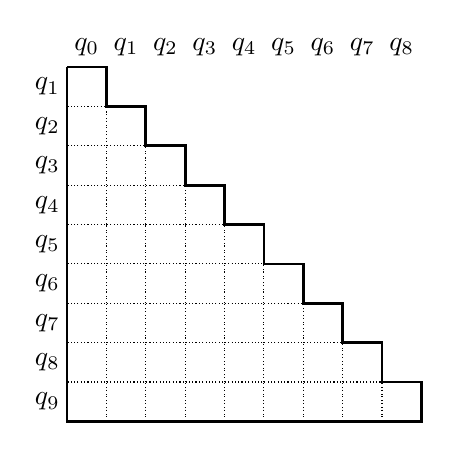
\begin{tikzpicture}[every node/.style={minimum width=0.5cm, minimum height=0.5cm, inner sep=0pt},x=0.5cm, y=0.5cm]
			% Rótulos das colunas (0 a 8)
			\foreach \j in {0,...,8} {
					\node at (\j + 0.5, 9.5) {$q_{\j}$};
			}
		
			% Rótulos das linhas (1 a 9)
			\foreach \i in {1,...,9} {
					\node at (-0.5, 9.5 - \i) {$q_{\i}$};
			}
		
			% Desenha a grade
			% Linhas de 1 a 9, Colunas de 0 a 8
			\foreach \i in {1,...,9} { % Linhas
					\foreach \j in {0,...,8} { % Colunas
							% A célula só existe se j < i
							% A célula (i,j) no seu diagrama corresponde a (\j, 9-\i) no sistema de coordenadas.
							% A borda diagonal segue a regra de que o número da coluna (j) deve ser menor que o número da linha (i)
							% ou seja, para uma matriz triangular inferior.
		
							% Ajuste para a forma do seu diagrama
							% A primeira linha (i=1) tem apenas a célula para j=0
							% A segunda linha (i=2) tem células para j=0, 1
							% E assim por diante, até a nona linha (i=9) com células para j=0 a 8
							\pgfmathsetmacro{\maxcol}{\i} % Para cada linha 'i', o número máximo de colunas é 'i'
							\ifnum\j < \maxcol % Verifica se a coluna está dentro dos limites para a linha atual
									\draw[dotted] (\j, 9-\i) rectangle (\j+1, 10-\i);
							\fi
					}
			}
		
			% Desenha a borda externa e a diagonal principal
			% As coordenadas foram ajustadas para corresponder aos rótulos e à forma
			\draw[line width=1pt]
				(0,9) -- (0,0) -- (9,0) % Base e lateral esquerda
				-- (9,1) -- (8,1) % Escalonamento da diagonal
				-- (8,2) -- (7,2)
				-- (7,3) -- (6,3)
				-- (6,4) -- (5,4)
				-- (5,5) -- (4,5)
				-- (4,6) -- (3,6)
				-- (3,7) -- (2,7)
				-- (2,8) -- (1,8)
				-- (1,9) -- (0,9); % Volta para o início
		
			% Adiciona os 'X's pretos (ajustando coordenadas para o novo sistema)
			% Coordenadas são (coluna + 0.5, 9 - linha + 0.5)
			\node at (0.5, 3.5) {$\checkmark$};
			\node at (1.5, 3.5) {$\checkmark$};
			\node at (2.5, 3.5) {$\checkmark$};
			\node at (3.5, 3.5) {$\checkmark$};
			\node at (4.5, 3.5) {$\checkmark$};
			\node at (5.5, 3.5) {$\checkmark$};

			\node at (0.5, 2.5) {$\checkmark$};
			\node at (1.5, 2.5) {$\checkmark$};
			\node at (2.5, 2.5) {$\checkmark$};
			\node at (3.5, 2.5) {$\checkmark$};
			\node at (4.5, 2.5) {$\checkmark$};
			\node at (5.5, 2.5) {$\checkmark$};

			\node at (0.5, 1.5) {$\checkmark$};
			\node at (1.5, 1.5) {$\checkmark$};
			\node at (2.5, 1.5) {$\checkmark$};
			\node at (3.5, 1.5) {$\checkmark$};
			\node at (4.5, 1.5) {$\checkmark$};
			\node at (5.5, 1.5) {$\checkmark$};

			\node at (0.5, 0.5) {$\checkmark$};
			\node at (1.5, 0.5) {$\checkmark$};
			\node at (2.5, 0.5) {$\checkmark$};
			\node at (3.5, 0.5) {$\checkmark$};
			\node at (4.5, 0.5) {$\checkmark$};
			\node at (5.5, 0.5) {$\checkmark$};
		\end{tikzpicture}
		\caption{Matriz de estados do AFD da Figura \ref{fig:AFDminimo1} candidatos a serem equivalentes.}
		\label{tab:AutomatoMinimo1}
	\end{figure}

	Todas as posições $(q_i, q_j)$ marcadas com {$\checkmark$} informam que os estados $q_i$ e $q_j$ foram detectados não equivalentes pelo Algoritmo \ref{alg:AFD-MatrizCandidatosEquivalentes}, em especial observe que os estados $q_0$ e $q_6$ de fato não podem ser equivalentes visto que $q_0 \notin F$ e $q_6 \in F$, por outro lado, como os estados $q_6, q_8 \in F$ eles são candidatos a serem equivalentes, então não existe uma marca na posição
correspondente, assim como também não há uma marca na posição referente aos estados $q_0$ e $q_2$. Passando o autômato e a matriz representada na Figura  \ref{tab:AutomatoMinimo1} para Algoritmo de Moore (Algoritmo \ref{alg:Moore}) tem-se que matriz será atualizada, ficando na forma abaixo.

	\begin{figure}[H]
		\centering
		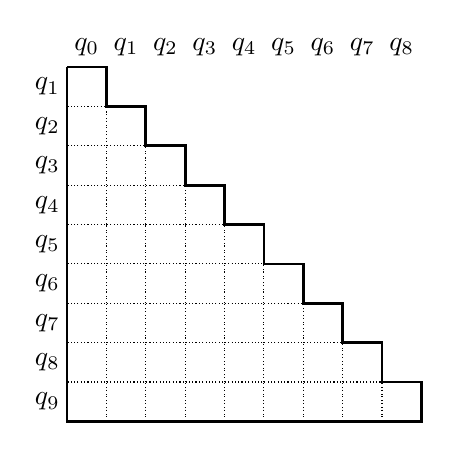
\begin{tikzpicture}[every node/.style={minimum width=0.5cm, minimum height=0.5cm, inner sep=0pt},x=0.5cm, y=0.5cm]
			% Rótulos das colunas (0 a 8)
			\foreach \j in {0,...,8} {
					\node at (\j + 0.5, 9.5) {$q_{\j}$};
			}
		
			% Rótulos das linhas (1 a 9)
			\foreach \i in {1,...,9} {
					\node at (-0.5, 9.5 - \i) {$q_{\i}$};
			}
		
			% Desenha a grade
			% Linhas de 1 a 9, Colunas de 0 a 8
			\foreach \i in {1,...,9} { % Linhas
					\foreach \j in {0,...,8} { % Colunas
							% A célula só existe se j < i
							% A célula (i,j) no seu diagrama corresponde a (\j, 9-\i) no sistema de coordenadas.
							% A borda diagonal segue a regra de que o número da coluna (j) deve ser menor que o número da linha (i)
							% ou seja, para uma matriz triangular inferior.
		
							% Ajuste para a forma do seu diagrama
							% A primeira linha (i=1) tem apenas a célula para j=0
							% A segunda linha (i=2) tem células para j=0, 1
							% E assim por diante, até a nona linha (i=9) com células para j=0 a 8
							\pgfmathsetmacro{\maxcol}{\i} % Para cada linha 'i', o número máximo de colunas é 'i'
							\ifnum\j < \maxcol % Verifica se a coluna está dentro dos limites para a linha atual
									\draw[dotted] (\j, 9-\i) rectangle (\j+1, 10-\i);
							\fi
					}
			}
		
			% Desenha a borda externa e a diagonal principal
			% As coordenadas foram ajustadas para corresponder aos rótulos e à forma
			\draw[line width=1pt]
				(0,9) -- (0,0) -- (9,0) % Base e lateral esquerda
				-- (9,1) -- (8,1) % Escalonamento da diagonal
				-- (8,2) -- (7,2)
				-- (7,3) -- (6,3)
				-- (6,4) -- (5,4)
				-- (5,5) -- (4,5)
				-- (4,6) -- (3,6)
				-- (3,7) -- (2,7)
				-- (2,8) -- (1,8)
				-- (1,9) -- (0,9); % Volta para o início
		
			% Adiciona os 'X's pretos (ajustando coordenadas para o novo sistema)
			% Coordenadas são (coluna + 0.5, 9 - linha + 0.5)
			\node at (0.5, 3.5) {$\checkmark$};
			\node at (1.5, 3.5) {$\checkmark$};
			\node at (2.5, 3.5) {$\checkmark$};
			\node at (3.5, 3.5) {$\checkmark$};
			\node at (4.5, 3.5) {$\checkmark$};
			\node at (5.5, 3.5) {$\checkmark$};

			\node at (0.5, 2.5) {$\checkmark$};
			\node at (1.5, 2.5) {$\checkmark$};
			\node at (2.5, 2.5) {$\checkmark$};
			\node at (3.5, 2.5) {$\checkmark$};
			\node at (4.5, 2.5) {$\checkmark$};
			\node at (5.5, 2.5) {$\checkmark$};

			\node at (0.5, 1.5) {$\checkmark$};
			\node at (1.5, 1.5) {$\checkmark$};
			\node at (2.5, 1.5) {$\checkmark$};
			\node at (3.5, 1.5) {$\checkmark$};
			\node at (4.5, 1.5) {$\checkmark$};
			\node at (5.5, 1.5) {$\checkmark$};

			\node at (0.5, 0.5) {$\checkmark$};
			\node at (1.5, 0.5) {$\checkmark$};
			\node at (2.5, 0.5) {$\checkmark$};
			\node at (3.5, 0.5) {$\checkmark$};
			\node at (4.5, 0.5) {$\checkmark$};
			\node at (5.5, 0.5) {$\checkmark$};

			\node[red] at (0.5, 7.5) {$\checkmark$}; % Linha 2, Coluna 0
			\node[red] at (1.5, 7.5) {$\checkmark$}; % Linha 2, Coluna 1
			\node[red] at (2.5, 6.5) {$\checkmark$}; % Linha 3, Coluna 2
			\node[red] at (0.5, 5.5) {$\checkmark$}; % Linha 4, Coluna 0
			\node[red] at (1.5, 5.5) {$\checkmark$}; % Linha 4, Coluna 1
			\node[red] at (3.5, 5.5) {$\checkmark$}; % Linha 4, Coluna 3
			\node[red] at (2.5, 4.5) {$\checkmark$}; % Linha 5, Coluna 2
			\node[red] at (4.5, 4.5) {$\checkmark$}; % Linha 5, Coluna 4
		\end{tikzpicture}
		\caption{Matriz de estados equivalentes do AFD da Figura \ref{fig:AFDminimo1}.}
		\label{tab:AutomatoMinimo2}
	\end{figure}

	Os símbolos $\checkmark$ vermelhos foram introduzido na execução do Algoritmo de Moore, agora com a tabela atualizada basta verificar as colunas para identificar os estados equivalentes, e assim construir as classes de equivalência, todos os estados (linhas) não marcado em um coluna $q_i$ são equivalentes ao estado $q_i$ assim pela matriz representada na Figura \ref{tab:AutomatoMinimo2} tem-se que,
	\begin{align*}
    [q_0] & = \{q_0, q_1, q_3, q_5\}\\
    [q_2] & = \{q_2, q_4\}\\
    [q_6] & = \{q_6, q_7, q_8, q_9\}
	\end{align*}
	e seguindo as regras para gerar a função de transição,
	\begin{align*}
			\delta([q_0], 1) & = [q_2]\\
			\delta([q_0], 0) & = [q_0]\\
			\delta([q_2], 1) & = [q_6]\\
			\delta([q_2], 0) & = [q_0]\\
			\delta([q_6], 1) & = [q_6]\\
			\delta([q_6], 0) & = [q_6]
	\end{align*}
	e $F_{/\equiv} = \{[q_6]\}$, assim tem-se AFD mínimo descrito na Figura \ref{fig:AFDminimo2}.

	\begin{figure}[H]
		\centering
		\begin{tikzpicture}[>=stealth, shorten >=1pt, node distance=2.5cm, on grid, auto, state/.append style={minimum size=2em}, thick ]
			\node[state, initial]				(0)               {$[q_0]$};
			\node[state]								(1) [right of=0] 	{$[q_2]$};
			\node[state, accepting]     (2) [right of=1] 	{$[q_6]$};
			\path[->] (0) +(-1,0) edge (0)
			
			%Transições:
			%(Partida) edge [tipo da seta] node {simbolo lido} (Destino)
			%(0) edge 			 				node [below] {$1$}		 (2)
			% [bend left] 
			(0) edge [loop above]	node {$0$}		 					( )
			(0) edge [bend left]  node {$1$}		 					(1)
			(1) edge [bend left]  node {$0$}		 					(0)
			(1) edge 			 				node {$1$}		 					(2)
			(2) edge [loop above]	node {$0,1$}	 					( );
		\end{tikzpicture}
		\caption{Um AFD.}
		\label{fig:AFDminimo2}
	\end{figure}
\end{exemplo}

\begin{exemplo}
	Considere o AFD representado pela Figura \ref{fig:AFDminimo3} a seguir.

	\begin{figure}[H]
		\centering
		\begin{tikzpicture}[>=stealth, shorten >=1pt, node distance=2.5cm, on grid, auto, state/.append style={minimum size=2em}, thick ]
			\node[state, initial]				(0)               {$q_0$};
			\node[state, accepting]			(1) [right of=0] 	{$q_1$};
			\node[state]     						(2) [right of=1] 	{$q_2$};
			\node[state]     						(3) [below of=0] 	{$q_3$};
			\node[state, accepting]			(4) [right of=3] 	{$q_4$};
			\node[state]     						(5) [right of=4] 	{$q_5$};
			\path[->] (0) +(-1,0) edge (0)
			
			%Transições:
			%(Partida) edge [tipo da seta] node {simbolo lido} (Destino)
			%(0) edge 			 				node [below] {$1$}		 (2)
			% [bend left] 
			(0) edge [bend left]  node {$1$}		 					(1)
			(0) edge [bend left]  node {$0$}		 					(3)
			(1) edge [bend left]  node {$1$}			 				(0)
			(1) edge [bend left]  node {$0$}			 				(2)
			(2) edge [bend left]  node {$0$}		 					(1)
			(2) edge [bend left]  node {$1$}		 					(5)
			(3) edge [bend left]  node {$1$}		 					(4)
			(3) edge [bend left]  node {$0$}		 					(0)
			(4) edge [bend left]  node {$1$}		 					(3)
			(4) edge [bend left]  node {$0$}		 					(5)
			(5) edge [bend left]  node {$0$}		 					(4)
			(5) edge [bend left]  node {$1$}		 					(2);
		\end{tikzpicture}
		\caption{Um AFD.}
		\label{fig:AFDminimo3}
	\end{figure}

	Usando o Algoritmo \ref{alg:AFD-MatrizCandidatosEquivalentes} é obtida a seguinte matriz de candidatos a estados equivalentes,

	\begin{figure}[H]
		\centering
		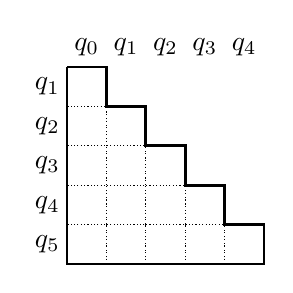
\begin{tikzpicture}[every node/.style={minimum width=0.5cm, minimum height=0.5cm, inner sep=0pt},x=0.5cm, y=0.5cm]
      % Rótulos das colunas (q_0 a q_4)
      \foreach \j in {0,...,4} {
          \node at (\j + 0.5, 5.5) {$q_{\j}$};
      }
    
      % Rótulos das linhas (q_1 a q_5)
      \foreach \i in {1,...,5} {
          \node at (-0.5, 5.5 - \i) {$q_{\i}$};
      }
    
      % Desenha a grade
      % Linhas de 1 a 5, Colunas de 0 a 4
      \foreach \i in {1,...,5} { % Linhas
          \foreach \j in {0,...,4} { % Colunas
              \pgfmathsetmacro{\maxcol}{\i}
              \ifnum\j < \maxcol
                  \draw[dotted] (\j, 5-\i) rectangle (\j+1, 6-\i);
              \fi
          }
      }
    
      % Desenha a borda externa e a diagonal principal
      \draw[line width=1pt]
          (0,5) -- (0,0) -- (5,0)
          -- (5,1) -- (4,1)
          -- (4,2) -- (3,2)
          -- (3,3) -- (2,3)
          -- (2,4) -- (1,4)
          -- (1,5) -- (0,5);
    
      % Coordenadas são (coluna + 0.5, 5 - linha + 0.5)
      %\node[red] at (0.5, 4.5) {$\checkmark$}; % Linha 1, Coluna 0
      %\node[red] at (1.5, 3.5) {$\checkmark$}; % Linha 2, Coluna 1
      %\node[red] at (0.5, 2.5) {$\checkmark$}; % Linha 3, Coluna 0
      %\node[red] at (2.5, 2.5) {$\checkmark$}; % Linha 3, Coluna 2

      %\node at (3.5, 0.5) {$\checkmark$}; % Linha 5, Coluna 3
      %\node at (4.5, 0.5) {$\checkmark$}; % Linha 5, Coluna 4


			\node at (0.5, 4.5) {$\checkmark$};
			\node at (0.5, 1.5) {$\checkmark$};

			\node at (1.5, 0.5) {$\checkmark$};
			\node at (1.5, 2.5) {$\checkmark$};
			\node at (1.5, 3.5) {$\checkmark$};

			\node at (2.5, 1.5) {$\checkmark$};

			\node at (3.5, 1.5) {$\checkmark$};

			\node at (4.5, 0.5) {$\checkmark$};
    \end{tikzpicture}
		\caption{Matriz de estados do AFD da Figura \ref{fig:AFDminimo3} candidatos a serem equivalentes.}
		\label{tab:AutomatoMinimo3}
	\end{figure}

	Aplicando a matriz representada pela Figura \ref{tab:AutomatoMinimo3} ao algoritmo de Moore tal matriz será atualizada para a forma a seguir.

	\begin{figure}[H]
		\centering
		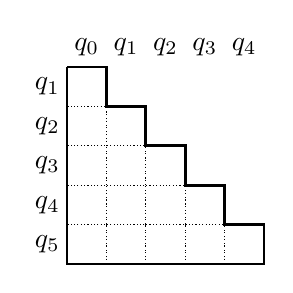
\begin{tikzpicture}[every node/.style={minimum width=0.5cm, minimum height=0.5cm, inner sep=0pt},x=0.5cm, y=0.5cm]
      % Rótulos das colunas (q_0 a q_4)
      \foreach \j in {0,...,4} {
          \node at (\j + 0.5, 5.5) {$q_{\j}$};
      }
    
      % Rótulos das linhas (q_1 a q_5)
      \foreach \i in {1,...,5} {
          \node at (-0.5, 5.5 - \i) {$q_{\i}$};
      }
    
      % Desenha a grade
      % Linhas de 1 a 5, Colunas de 0 a 4
      \foreach \i in {1,...,5} { % Linhas
          \foreach \j in {0,...,4} { % Colunas
              \pgfmathsetmacro{\maxcol}{\i}
              \ifnum\j < \maxcol
                  \draw[dotted] (\j, 5-\i) rectangle (\j+1, 6-\i);
              \fi
          }
      }
    
      % Desenha a borda externa e a diagonal principal
      \draw[line width=1pt]
          (0,5) -- (0,0) -- (5,0)
          -- (5,1) -- (4,1)
          -- (4,2) -- (3,2)
          -- (3,3) -- (2,3)
          -- (2,4) -- (1,4)
          -- (1,5) -- (0,5);
    
      % Coordenadas são (coluna + 0.5, 5 - linha + 0.5)
      %\node[red] at (0.5, 4.5) {$\checkmark$}; % Linha 1, Coluna 0
      %\node[red] at (1.5, 3.5) {$\checkmark$}; % Linha 2, Coluna 1
      %\node[red] at (0.5, 2.5) {$\checkmark$}; % Linha 3, Coluna 0
      %\node[red] at (2.5, 2.5) {$\checkmark$}; % Linha 3, Coluna 2

      %\node at (3.5, 0.5) {$\checkmark$}; % Linha 5, Coluna 3
      %\node at (4.5, 0.5) {$\checkmark$}; % Linha 5, Coluna 4


			\node at (0.5, 4.5) {$\checkmark$};
			\node[red] at (0.5, 3.5) {$\checkmark$};
			\node at (0.5, 1.5) {$\checkmark$};
			\node[red] at (0.5, 0.5) {$\checkmark$};

			\node at (1.5, 0.5) {$\checkmark$};
			\node at (1.5, 2.5) {$\checkmark$};
			\node at (1.5, 3.5) {$\checkmark$};

			\node at (2.5, 1.5) {$\checkmark$};
			\node[red] at (2.5, 2.5) {$\checkmark$};

			\node at (3.5, 1.5) {$\checkmark$};
			\node[red] at (3.5, 0.5) {$\checkmark$};

			\node at (4.5, 0.5) {$\checkmark$};
    \end{tikzpicture}
		\caption{Matriz de estados equivalentes do AFD da Figura \ref{fig:AFDminimo3}.}
		\label{tab:AutomatoMinimo4}
	\end{figure}

	Agora usando as regras de construção do AFD quociente após a aplicação do algoritmo de Moore ficamos com as seguintes classes de equivalência.
	\begin{align*}
    [q_0] & = \{q_0, q_3\}\\
    [q_1] & = \{q_1, q_4\}\\
    [q_2] & = \{q_2, q_5\}
	\end{align*}
	e seguindo as regras para gerar a função de transição tem-se,
	\begin{align*}
			\delta([q_0], 1) & = [q_1]\\
			\delta([q_0], 0) & = [q_0]\\
			\delta([q_1], 1) & = [q_0]\\
			\delta([q_1], 0) & = [q_2]\\
			\delta([q_2], 1) & = [q_2]\\
			\delta([q_2], 0) & = [q_1]
	\end{align*}

	Logo o AFD quociente e da forma descrita pela Figura \ref{fig:AFDminimo4} a seguir.

	\begin{figure}[H]
		\centering
		\begin{tikzpicture}[>=stealth, shorten >=1pt, node distance=2.5cm, on grid, auto, state/.append style={minimum size=2em}, thick ]
			\node[state, initial]				(0)               {$[q_0]$};
			\node[state, accepting]			(1) [right of=0] 	{$[q_1]$};
			\node[state]     						(2) [right of=1] 	{$[q_2]$};
			\path[->] (0) +(-1,0) edge (0)
			
			%Transições:
			%(Partida) edge [tipo da seta] node {simbolo lido} (Destino)
			%(0) edge 			 				node [below] {$1$}		 (2)
			% [bend left] 
			(0) edge [bend left]  node {$1$}		 					(1)
			(0) edge [loop above]	node {$0$}		 					( )
			(1) edge [bend left]  node {$1$}			 				(0)
			(1) edge [bend left]  node {$0$}			 				(2)
			(2) edge [bend left]  node {$0$}		 					(1)
			(2) edge [loop above]	node {$1$}		 					( );
		\end{tikzpicture}
		\caption{Um AFD.}
		\label{fig:AFDminimo4}
	\end{figure}
\end{exemplo}

Agora será apresentado o algoritmo de Hopcroft \cite{hopcroft1971} para minimiza um AFD dado, a ideia de Hopcroft é realizar o refinamento progressivo das partições do conjunto de estados, usando a ideia de blocos \sidefootnote{Que em última análise serão classes de equivalência}. O conceito é quebrar o conjunto de estados em subconjuntos contendo apenas estados equivalentes.	

\begin{definicao}
	Seja $A = \langle Q, \Sigma, \delta, q_0, F\rangle$ um AFD, um bloco é qualquer $X \subseteq Q$ tal que todos os $q_i \in X$ são do mesmo tipo\footnote{Tipo aqui corresponde a mesma ideia do algoritmo de Moore, ou seja, o tipo de estados finais e não-finais.}.
\end{definicao}


\section{Questionário}\label{sec:Questionario2part1}


\begin{questao}\label{exer:AF1}
	Para cada linguagem a seguir construa um AFD.
\end{questao}

\begin{exerList}
	\item $L_1 = \{w \in \{a,b\}^* \mid w \text{ termina em } ab\}$.
  \item $L_2 = \{w \in \{0, x, 1\}^* \mid w \text{ começa com } 1 \text{ mas não contém a subpalavra } 0xx1 \}$.
  \item $L_3 = \{w \in \{1, 2, 0\}^* \mid w \text{ contém a subpalavra } 1201\}$.
  \item $L_4 = \{w \in \{a,b\}^* \mid w = a^n \text{ com } n \in \mathbb{N} \text{ ou se existe } b \text{ em } w \text{, ele é seguido de aa}\}$.
  \item $L_5 = \{w \in \{0,1\}^* \mid w \text{ não possui nem uma subpalavra } 0^{2n} \text{ com } n \in \mathbb{N}\}$.
  \item $L_6 = \{w \in \{a,b, c\}^* \mid w \in \{b, c\}^* \text{ ou } \text{ todo } a \text{ em } w \text{ aparece entre } b \text{ e } c\}$.
\end{exerList}

\begin{questao}\label{exer:AF2}
	Para cada linguagem a seguir construa um AFD, AFN ou $\lambda$-AFN que reconhecer a linguagem. Considerando que $N_a(w)$ corresponde ao número de $a \in \Sigma$ na palavra $w$.
\end{questao}

\begin{exerList}
	\item $L_1 = \{w \in \{\circ, \star, 0, 1\}^* \mid N_\star(w) > 3 \land N_\circ(w) < 5\}$.
  \item $L_2 = \{w \in \{0, x, 1\}^* \mid w N_x(w) = 6\}$.
  \item $L_3 = \{u0^i1^jv \in \{1, 2, 0\}^* \mid u, v \in \{2\}^* \land  i + j = 2k + 1, k \in \mathbb{N}-\{0\}\}$.
	\item $L_4 = \{ubv \mid u, v \in \{a, b, c\}^*, N_b(u) = 0 \land N_b(v) < 5\}$.
\end{exerList}

\begin{questao}\label{exer:AF3}
	Considere que $\Sigma = \{0, 1\}$, para cada linguagem a seguir construa um AFD, AFN ou $\lambda$-AFN que reconhecer a linguagem descrita.
\end{questao}

\begin{exerList}
	\item A linguagem de todas as palavras começando com $0$ e terminando com $1$ e que não apareça a sub-palavra $01010$.
	\item A linguagem de todas as palavras começando com $10$ e que não possuem a sub-palavra $001$.
	\item A linguagem de todas as palavras terminando com $(11)^2$ ou $(11)^4$. 
	\item A linguagem de todas as palavras que possuem as sub-palavras $010$ ou $101$.
\end{exerList}

\begin{questao}\label{exer:AF4}
	Considere que $\Sigma = \{a, b, c, d\}$ construa um AFD que reconhece a linguagem de todos os $w \in \Sigma^*$ tal que $w$ satisfaz as seguintes restrições.
	\begin{itemize}
		\item[(i)] $w$ nunca deve conter a subpalavra $abcd$;
		\item[(ii)] Sempre que $w$ iniciar em $a$ obrigatoriamente deve terminar $cd$;
		\item[(iii)] Se $w$ iniciar com $b$ então não deve conter a subpalavra $bc$ e 
		\item[(iv)] $w$ sempre contém a subpalavra $ac$.  
	\end{itemize}
\end{questao}


\begin{questao}\label{exer:AF5}
	Considere que $\Sigma = \{0, 1\}$ construa um AFD que reconhece a linguagem de todos os $w \in \Sigma^*$ tal que $w$ satisfaz as seguintes restrições.
	\begin{itemize}
		\item[(i)] Sempre que $w$ iniciar com $00$ tem-se que $|w| < 10$;
		\item[(ii)] Sempre que $w$ iniciar em $10$ obrigatoriamente deve terminar $00$;
		\item[(iii)] Se $w$ iniciar com $01$ não deve conter a subpalavra $101$ e 
		\item[(iv)] $w$ sempre deve ter tamanho par.  
	\end{itemize}
\end{questao}

\begin{questao}\label{exer:AF6}
	Considere que $\Sigma = \{0, 1\}$ construa um AFD que reconhece a linguagem de todos os $w \in \Sigma^*$ tal que $w$ satisfaz as seguintes restrições.
	\begin{itemize}
		\item[(i)] $w$ nunca inicia com $00$ ou $11$;
		\item[(ii)] Sempre que $w$ deve possuir a subpalavra $101$ e também deve possuir a subpalavra $010$;
		\item[(iii)] Em $w$ subpalavra $101$ e sempre aparece antees da subpalavra $010$;
	\end{itemize}
\end{questao}




\begin{questao}\label{exer:AFx}
	Seja $L \subseteq \Sigma$ para um alfabeto $\Sigma$ qualquer com $\# \in \Sigma$, demonstre que todas as linguagens a seguir são regulares.
\end{questao}

\begin{exerList}
	\item $L_1 = \{\#^{|w|} \in \Sigma^* \mid w \in L\}$.
	\item $L_2 = \{d_{\#}(w) \in \Sigma^* \mid w \in L\}$, onde $d_{\#}(w)$ corresponde a uma palavra $w' \in \Sigma^*$, de forma que $w'$ é a forma reduzida de $w$ após remover todos os $\#$.
	\item $L_3 = \{x \in \Sigma^* \mid x,y \in L \land y \in \Sigma^*\}$.
	\item $L_4 = \{y \in \Sigma^* \mid x,y \in L \land x \in \Sigma^*\}$.
	\item $L_5 = \{x \in \Sigma^* \mid x,y \in L \land x \in \Sigma^*\}$.
	\item $L_6 = \{xy \in \Sigma^* \mid x,y \in \Sigma^* \land yx \in L\}$.
	\item $L_7 = \{w \in \Sigma^* \mid www \in L\}$.
	\item $L_8 = \{x \in L \mid xy \in L \Longleftrightarrow y = \lambda\}$.
	\item $L_9 = \{xy \in L \mid y \in L \Longleftrightarrow x = \lambda\}$.
\end{exerList}